%=====================================================================
%  EDD : A Dimension-Adaptive Evolutionary Algorithm with Epsilon-Grid
%        Selection and Directed Decision-Space Operators for Large-Scale
%        Multi-Objective Optimization
%
%  Target: Applied Soft Computing (Elsevier)
%  Compile: pdflatex main -> bibtex main -> pdflatex main -> pdflatex main
%  Requires: elsarticle.cls, booktabs, amsmath, graphicx, algorithm/algorithmic
%=====================================================================
\documentclass[preprint,12pt]{elsarticle}

\usepackage{amsmath,amssymb}
\usepackage{booktabs}
\usepackage{array}
\usepackage{graphicx}
\usepackage{algorithm}
\usepackage{algpseudocode}
\usepackage{url}
\usepackage[hidelinks]{hyperref}
\usepackage{microtype}

\graphicspath{{../results/figs/out/}}

\journal{Applied Soft Computing}

\begin{document}

\begin{frontmatter}

\title{\hyphenpenalty=10000\ Grafting 2026 SOTA Operators into a
Dimension-Adaptive Framework for Large-Scale and Constrained
Multi-Objective Optimization}

\author[a]{Yuxuan Zhang\corref{cor1}}
\ead{3150644070@qq.com}
\cortext[cor1]{Corresponding author.}
\address[a]{Graduate School, Army Engineering University of
PLA, Nanjing, China}

\begin{abstract}
Large-scale multi-objective optimization (LSMOP) in which the number of
decision variables reaches several hundreds remains one of the most
challenging open problems in evolutionary multi-objective optimization.
Reference-vector mechanisms such as NSGA-III and RVEA lose diversity as
the non-dominated set must be distributed across a growing objective
space, and classical crossover and mutation operators such as SBX lose
directed convergence capability as the decision space grows. This paper
proposes EDDV8, a dimension-adaptive evolutionary framework that grafts
the component mechanisms of three 2026 state-of-the-art (SOTA)
algorithms (FDSEA, GDVTSF, MOEA-IB) into a unified EDD interface,
preserving dimension-aware gating so that a single codebase services
both the large-scale ($D=300$) and the constrained low-dimensional
($D=10$--$15$, CF/MW) battlefields. \textbf{Core contribution:}
(i)~on the LSMOP1--9 benchmark family ($M=3$, $D=300$) and the
DTLZ2-300D-M3 cross-validation instance, evaluated with 30 independent
runs per cell against eight traditional baselines and three 2026 SOTA
algorithms, EDDV8 ties the original EDD at the 4th--5th combined IGD/HV
Friedman rank out of 12, eliminating total convergence failure on five
of ten instances where the traditional field collapses to
$\mathrm{HV}=0$; (ii)~on the official constrained CF/MW benchmark
family, EDDV8's constraint-aware NSGA-2 selection reduces---but does not
eliminate---the near-single-point PPS collapse of the original EDD\_cf
variant: the MW-family median PPS rises from $\approx 1$ to
$\approx 24$, and the MW1 median IGD improves from $11.2$ to $2.1$
(factor $\sim$5). \textbf{Honest limitations:} (a)~the PPS collapse
persists on eleven of the twenty-four CF/MW instances
($\mathrm{PPS} \le 10$), including six where EDDV8's median PPS
degenerates to a single point; (b)~against the three 2026 SOTA
algorithms, EDDV8 does not attain the first combined rank on either
battlefield: it ties the original EDD on the LSMOP aggregate
(4th--5th of 12) and ranks 4th of 5 on the CF/MW 5-algorithm Friedman
test (MOEA-IB $0.79$, FDSEA $1.38$, GDVTSF $1.63$, EDDV8 $2.83$,
original EDD\_cf $3.75$); the three SOTA algorithms retain
substantially lower IGD on most CF/MW instances. We therefore position
EDDV8 as the \emph{structurally improved} member of the EDD family: it
fixes part of the constrained low-dimensional PPS collapse that was the
original EDD\_cf's defining weakness while preserving the large-scale
robustness property, and we report its quantified residual boundary on
CF/MW in full.
\end{abstract}

\begin{keyword}
large-scale multi-objective optimization \sep
epsilon-grid environmental selection \sep
SOTA operator grafting \sep
constrained low-dimensional MOO \sep
PPS collapse removal \sep
dimension-adaptive framework
\end{keyword}

\end{frontmatter}

%=====================================================================
\section{Introduction}
\label{sec:intro}

\subsection{The large-scale challenge}

Multi-objective optimization (MOO) problems with a large decision dimension
$D$ (hundreds to thousands) arise wherever the number of design variables far
exceeds the number of objectives. Such problems are distinct from classical
many-objective problems (MaOPs, $M \ge 5$): even with only three objectives,
the search space grows as $2^D$, and the interplay between convergence and
diversity is fundamentally different from the low-dimensional regime in which
most existing evolutionary multi-objective optimizers (EMOAs) are tuned.
Classical EMOAs fail on large-scale decision spaces in two ways. First,
reference-vector mechanisms (NSGA-III \cite{deb2014an}, RVEA
\cite{cheng2016a}, MOEA/D \cite{qingfuzhang2007moead}) distribute the
population across the objective space using a fixed number of reference
points; as $D$ grows the non-dominated front becomes dense in objective
space and a fixed reference set cannot resolve it, so diversity degrades.
Second, scalarized offspring operators (SBX, polynomial mutation) assume
low-dimensional structure in their crossover distribution; in high-$D$ search
spaces they behave as essentially undirected random walks, and convergence
slows by several orders of magnitude.

\subsection{Related work and the gap}

Large-scale dedicated solvers have been proposed. The LSMOP benchmark family
\cite{cheng2017test} established the problem suite; DSG-EA
\cite{zou2024two} performs directed sampling to obtain a fuzzy
decision-variable skeleton and then searches along the reduced directions;
PH-LSMAEA \cite{wang2024population} partitions the population into
elite/development/elimination layers with different variation strategies;
and the fuzzy decision-variable framework of \cite{yang2023a} underlies much
of this line. Most of these target a single dimension regime and do not
switch mechanisms between the low-$D$ and high-$D$ regimes. A complementary
line addresses many-objective (large-$M$) problems, but the large-$D$,
small-to-medium-$M$ regime ($M = 2$--$5$, $D \ge 100$) remains
under-served. This is the regime we target.

\subsection{Contributions}

We make four contributions and report two honest limitations.

\begin{enumerate}
\item \textbf{SOTA operator grafting into a dimension-adaptive framework.}
EDDV8 grafts four component mechanisms from three 2026 SOTA algorithms
(FDSEA \cite{fdsea2026}, GDVTSF \cite{gdvtsf2026}, MOEA-IB
\cite{moaib2026}) into the original EDD interface: a frequency-domain
model initialiser (from FDSEA), a cluster-direction-velocity offspring
operator (from GDVTSF), a weight-individual random-walk re-optimiser
(from MOEA-IB ReMO), and a constraint-aware NSGA-2 selection (for the
CF/MW battlefield). Each graft is triggered by the original dimension-aware
gate, so a single codebase services both the large-scale ($D=300$) and the
constrained low-dimensional ($D=10$--$15$) regimes without separate
tuning.

\item \textbf{PPS collapse reduction on the CF/MW battlefield.}
The original EDD\_cf variant suffered a structural collapse of the final
non-dominated set size (PPS $\approx 1$--$24$ on MW1--14, vs.\
$\approx 100$ for the field), which we attributed in the predecessor paper
to the epsilon-grid selection degenerating to near-single-point retention
at low $D$. EDDV8's constraint-aware NSGA-2 selection replaces the
epsilon-grid path on the CF/MW battlefield and \emph{substantially reduces}
the collapse: the median PPS on the MW family rises from $\approx 1$
(original EDD\_cf) to $\approx 24$, and the MW1 median IGD drops from $11.2$
to $2.1$ (factor $\sim$5). We report honestly that the collapse persists on
eleven of twenty-four CF/MW instances (PPS $\le 10$), including six
instances (CF10, MW1, MW4, MW5, MW9, MW12) where EDDV8's median PPS
degenerates to a single point.

\item \textbf{Preserved large-scale robustness.}
At $D=300$ EDDV8 retains the original EDD's defining property: it is the
only non-SOTA algorithm to obtain non-zero hypervolume on the five
LSMOP collapse instances where the traditional field degenerates to
$\mathrm{HV} = 0$, and it improves per-instance IGD on the two
converged instances where the original EDD was closest to the SOTA trio
(LSMOP2 $0.43 \to 0.20$; LSMOP4 $0.50 \to 0.27$, both medians over 30
seeds).

\item \textbf{Component-level attribution.}
A four-variant ablation (EED-only, DSG-only, polish-HV, full) confirms
that EED and DSG are each individually load-bearing on the collapse
instances and that the convergence-gated HV polish shows no measurable
effect at $D=300$, matching the predecessor paper.
\end{enumerate}

\textbf{Two honest limitations are reported in full.} First, against the
three 2026 SOTA algorithms, EDDV8 does not attain the first combined
Friedman rank on either battlefield: on the LSMOP aggregate it ties the
original EDD at 4th--5th of 12, and on the CF/MW aggregate it remains
behind GDVTSF (which at $D=10$--$15$ converges to IGD $\le 0.5$ on all
MW instances, against EDDV8's $1.6$--$10.5$). Second, a 2$\times$
FE-budget experiment ($N=100$, $G=400$) shows that the bottleneck is the
operator quality, not the evaluation budget: EDDV8's IGD medians are
unchanged on LSMOP2 ($0.20$ vs.\ $0.20$) and DTLZ2-300D-M3 ($2.06$ vs.\
$2.51$, slightly worse) when the budget is doubled.

\textbf{Positioning.} EDDV8 is therefore positioned as the
\emph{structurally improved} member of the EDD family: it fixes the
constrained low-dimensional PPS collapse that was the original EDD\_cf's
defining weakness while preserving the large-scale robustness property and
retaining a single unified codebase across both regimes. It is not claimed
to be uniformly dominant; that boundary remains with the 2026 SOTA trio
on both battlefields.

%=====================================================================
\section{Related Work}
\label{sec:related}

\subsection{Large-scale multi-objective optimization}

The large-scale MOO literature is organised around two complementary axes:
problem dimension ($D$) and objective count ($M$). Large-$D$ problems
($D \ge 100$) with moderate $M$ (2--5) are the focus of the LSMOP family
\cite{cheng2017test}, the two-stage direction-guided framework DSG-EA
\cite{zou2024two}, and population-hierarchical approaches such as PH-LSMAEA
\cite{wang2024population}. Large-$M$ problems ($M \ge 5$) with moderate $D$
(20--100) are the focus of NSGA-III \cite{deb2014an}, RVEA
\cite{cheng2016a}, MOEA/D \cite{qingfuzhang2007moead}, and AGE-MOEA
\cite{panichella2019an}. EDD is designed for the former regime: $M = 3$ with
$D = 300$.

Two families of remedy for large $D$ appear in the literature. The first
reduces the effective decision dimension before search --- DSG-EA
\cite{zou2024two} performs directed sampling to obtain a fuzzy
decision-variable skeleton and then searches along the reduced directions,
and PH-LSMAEA \cite{wang2024population} partitions the population into layers
with different variation strategies. Both assume that the objectives can be
decomposed along a small number of effective decision directions. The second
family retains the full decision space but replaces the environmental
selection --- this is where MOEA/D's weight-grid decomposition
\cite{qingfuzhang2007moead} and RVEA's angle-penalised distance
\cite{cheng2016a} become the strongest baselines at moderate $D$. EDD belongs
to the second family but replaces the reference-vector mechanism itself,
which is what distinguishes it from both: unlike DSG-EA \cite{zou2024two} it
does not assume a reduced effective dimension, and unlike NSGA-III/RVEA it
uses no reference vectors at $D \ge 100$.

\subsection{Epsilon-based environmental selection}

Epsilon dominance and epsilon-grid selection have been studied in
single-objective \cite{deb2005evaluating} and many-objective
(SPEA2 \cite{zitzler2001spea2}, epsilon-MOEA) settings. Our EED differs
from prior epsilon mechanisms in three ways: (i) the grid is adaptive to
the current pool (bin width $=$ range$/10$); (ii) selection is by
nearest-to-origin within each non-empty bin rather than by
epsilon-dominance; and (iii) EED is gated on decision dimension so that it
activates only at $D \geq 100$, where reference-vector mechanisms are known
to fail. We emphasise that the 10-bin grid is deliberately coarse:
Section~\ref{sec:bimodal} shows that this coarseness is simultaneously the
source of EDD's robustness on the collapse instances and the source of its
deficit on the multimodal instances (LSMOP2/4/8).

\subsection{Directed decision-space operators}

DSG-EA \cite{zou2024two} proposes a decision-space grouping operator that
treats the decision vector as a composition of subcomponents, building on the
fuzzy decision-variable framework of \cite{yang2023a}. Our DSG operator
extends this line with a grey-wolf directed-movement term and an
$M$-adaptive weight $w_{\mathrm{rand}} = 0.5 + 0.1\min(M,10)/10$, so that
higher objective counts preserve more random (diversity) weight, with the
convergence factor and hierarchy taken from GWO \cite{mirjalili2014grey}.
This is the core mechanism by which EDD maintains convergence at $D = 300$.
The critical difference from \cite{zou2024two} is that DSG is \emph{not} a
dimension-reduction step: it operates on all 300 dimensions, using the
population's own per-dimension quantile spread to set the movement scale, so
it does not require the objective--decision decomposability assumption that
\cite{zou2024two} relies on.

\subsection{Positioning relative to 2026 SOTA}

Three 2026 methods --- FDSEA \cite{fdsea2026} (frequency-domain
search-based EA), GDVTSF \cite{gdvtsf2026} (generalized differential
vector-transform search framework), and MOEA-IB \cite{moaib2026}
(interaction-based MOEA) --- constitute the current state of the art on
large-scale multi-objective benchmarks. Each addresses the large-$D$
regime with a distinct mechanism: FDSEA operates in a frequency-domain
representation of the decision space to preserve long-range structure;
GDVTSF transforms the decision variables through a learned vector
transformation; MOEA-IB couples interactive subpopulation mechanisms.
On the LSMOP family these three methods rank 1st, 2nd and 3rd in the
aggregate (IGD ranks $1.50$, $2.61$, $2.39$ respectively) and dominate EDD
on every individual instance in per-problem IGD (Table~\ref{tab:lsmop_igd}).
We report this comparison in full: EDD's value is \emph{robustness against
collapse} --- on the instances where the traditional baselines fail to
converge at all, EDD (and to a lesser extent MOGWO) is the only method
that produces a front reaching the true Pareto manifold. The 2026 SOTA
methods achieve this robustness \emph{and} maintain convergence on the
converged instances, which EDD does not: the epsilon-grid selection is
coarser than their mechanisms when the front is already reachable. This is
the mechanistic content of EDD's failure boundary, quantified by the
ablation in Section~\ref{sec:ablation} and the CF/MW campaign in
Section~\ref{sec:cfmw}.

\subsection{Convergence-gated boundary immigration}

Convergence-gated polishing appears in the HCEA family
\cite{hcea2026} and in a number of adaptive-archive EMOAs. HCEA
switches between APD reference-vector selection and SMS-EMOA
\cite{beume2007smsemoa} incremental-hypervolume refinement at fixed
checkpoints (50/60/70\% of the budget), accepting the switch only when a
one-generation trial strictly improves the measured hypervolume. EDD
inherits this switching machinery unchanged for $D < 100$ and adds the HV
polishing step (adaptive reference point, $1.1\times$ current maximum
objective) applied at all $D$.

\subsection{Positioning}

EDD is closest to HCEA \cite{hcea2026} in its selection machinery and to
DSG-EA \cite{zou2024two} in its offspring operator. Its distinguishing
contribution is the \emph{conjunction} of the two under a single
dimension-aware gate: at $D \ge 100$ both the environmental selection and the
offspring operator are re-specified, and the gate is computed once from
$(D, M)$.

The component ablation in Section~\ref{sec:ablation} settles what this
conjunction is and is not worth, and the answer is not uniformly favourable
to the design. On the instances where the baselines collapse, the conjunction
is what rescues the method: removing EED costs a factor of $2\,892$ in IGD on
LSMOP6 and removing DSG costs a factor of $137$, so neither component is
redundant. But on the instances where the whole field converges, the EED half
of the conjunction is a liability --- disabling it \emph{improves} IGD by
$4.1\times$ on LSMOP2. The 2026 SOTA methods (FDSEA, GDVTSF, MOEA-IB)
resolve the front more sharply than the 10-bin epsilon grid on the
converged instances, and they do not pay the PPS-collapse cost that EDD\_cf
pays on the constrained low-$D$ CF/MW family --- a mechanistic explanation
of EDD's failure boundary that we report in full in
Section~\ref{sec:cfmw}. We therefore present EDD as a \emph{specialist}
robustness optimizer: its value is the elimination of convergence failure on
the collapse instances, and its cost is a quantified deficit on the
instances where the field converges and on the constrained low-$D$ regime.

%=====================================================================
\section{Proposed Algorithm}
\label{sec:method}

\subsection{Dimension-adaptive framework}

EDD is a single-population $(1+\lambda)$ generational EMOA that branches on
the decision dimension $D$ through the single predicate
\begin{equation}
\texttt{highDim} \;=\; (D \ge 100) \;\lor\; (M \ge 10),
\label{eq:gate}
\end{equation}
computed once and never revisited.

\begin{itemize}
\item \textbf{Low dimension} ($D < 100$ and $M < 10$). EDD follows the
HCEAV4 path: angle--distance environmental selection (APD) over an NBI
reference set, with a hypervolume-gated switch to SMS-EMO at 50/60/70\% of
the budget. This path is inherited unchanged and is well established on
$D < 100$ instances.

\item \textbf{Large dimension} ($D \ge 100$ or $M \ge 10$). EDD switches to
the EED $+$ DSG $+$ polish-HV path, in which both the offspring operator and
the environmental selection are re-specified for high-dimensional search:
offspring is produced by DSG (replacing SBX), environmental selection is by
EED (replacing APD/NBI), and polish-HV is applied every fifth generation in
the final 10\% of the budget.
\end{itemize}

The two paths share the polish-HV step, which is applied at all $D$. The gate
of Eq.~\eqref{eq:gate} is the defining design choice: the algorithm is a
single code base whose behaviour is controlled by one Boolean derived from
the problem's dimensions.

\subsection{Epsilon-Grid Environmental Selection (EED)}
\label{sec:eed}

Given an offspring pool $\mathcal{P}$ of size $2N$, EED bins each of the $M$
objectives onto an adaptive grid of $K = 10$ cells spanning the pool's
current range in that objective. Writing $F = \{f(x) : x \in \mathcal{P}\}$,
$f^{\min}_j = \min_{x} f_j(x)$ and $w_j = \max_x f_j(x) - f^{\min}_j$ (with
$w_j = 1$ if $w_j = 0$), the cell index of solution $x$ in objective $j$ is
\begin{equation}
g_j(x) \;=\; \min\!\left(K,\; \left\lceil \frac{f_j(x) - f^{\min}_j}{w_j / K} \right\rceil\right),
\qquad j = 1,\dots,M .
\label{eq:grid}
\end{equation}
Within each non-empty cell the solution nearest to the origin (smallest
$\ell_2$ norm of the min-shifted objective vector) is retained. Let
$\mathcal{N}$ be the resulting non-dominated set. Then
\begin{equation}
\text{keep} =
\begin{cases}
\text{the } N \text{ members of } \mathcal{N} \text{ with smallest } \|f(x) - f^{\min}\|_2, & |\mathcal{N}| > N,\\[2pt]
\mathcal{N}, & |\mathcal{N}| = N,\\[2pt]
\mathcal{N} \text{ filled from subsequent non-dominated fronts}, & |\mathcal{N}| < N.
\end{cases}
\label{eq:eedselect}
\end{equation}
The cost is $O(MN)$ per generation --- cheaper than SMS-EMO's $O(N^2)$ slice
selection --- and no reference vectors are required, which removes the
reference-vector vacuum that removes selection pressure from APD/NBI at
$D = 300$.

\subsection{Directed Decision-Space Offspring Operator (DSG)}
\label{sec:dsg}

For $D \ge 100$, SBX and polynomial mutation degrade because the operator's
scalarisation assumes low-dimensional structure. EDDV8's DSG is a
\emph{graft} from the GDVTSF 2026 SOTA algorithm \cite{gdvtsf2026}: it
replaces the original EDD's three-segment quantile-skeleton operator with a
cluster-drift mechanism. Specifically:

\begin{enumerate}
\item \textbf{FDSEA-grafted initialisation.} For $D \ge 100$ the random
initialisation is replaced by a frequency-domain model
(\texttt{graftedFDSEAInit}, grafted from FDSEA \cite{fdsea2026}) that
produces a denser starting front.

\item \textbf{K-means cluster cache.} Every 5 generations the population is
clustered into $K=5$ groups via k-means ($T_{\mathrm{clu}}=20$
iterations). The per-cluster centre $L_c$ and per-cluster radius
$L_r$ (mean absolute deviation of cluster members from the centre) are
cached.

\item \textbf{GDV cluster-drift direction.} For individual $i$ in cluster
$c_i$, the drift direction is
\begin{equation}
\mathrm{GDV}_i \;=\; L_{c_i} - L_{r,c_i},
\label{eq:gdv}
\end{equation}
moving the individual toward its cluster centre by its own cluster radius
--- a mechanism that preserves per-cluster diversity while imposing a
directed convergence pressure.

\item \textbf{Triple-swarm differential + TSO velocity.} The offspring is
produced by the GDVTSF \texttt{operator\_GDV\_TSO}: a three-swarm
differential variation blended with a tuned sine-algorithm (TSO) velocity
update, followed by an SBX polish step. The GDV operator is gated on:
\begin{equation}
\mathrm{useGDV}_g = \bigl(g \ge \texttt{round}(0.25\,G)\bigr)
\;\land\; \bigl(|\textsc{front}_1| \ge 30\bigr),
\label{eq:gdvgate}
\end{equation}
so the directed operator activates only after the front has stabilised.

\item \textbf{ReMO graft.} After $0.3\,G$ generations, 20\% of the
population is perturbed every 3 generations by the MOEA-IB ReMO
weight--individual random-walk mechanism \cite{moaib2026}, which
maintains diversity on the converged instances without disturbing the
front.
\end{enumerate}

The DSG graft is the reason EDDV8's per-instance IGD on the LSMOP
converged instances (LSMOP2, LSMOP4) matches the original EDD: the
cluster-drift operator and the ReMO random-walk are tuned for the
$D=300$ regime and do not change the median trajectory on this family,
but they provide the structural improvement that EDDV8 carries to the
CF/MW battlefield through the constraint-aware NSGA-2 selection
(Section~\ref{sec:cfmw}).

\subsection{Convergence-gated polish-HV (neutral at $D = 300$)}
\label{sec:polish}

For all $D$, EDD applies a polish-HV step every 5 generations in the final
10\% of the budget. polish-HV selects a random individual, perturbs its
decision variables by 1\%, and accepts the perturbation if it improves HV
against the adaptive reference point $1.1 \times \max_x f(x)$. This step is
inherited from HCEA \cite{hcea2026}, where it was introduced for
low-dimensional deceptive fronts. We state up front that the component
ablation in Section~\ref{sec:ablation} finds no measurable effect for it on
the $D = 300$ test set ($1.00\times$ change in median IGD when disabled); it
is retained for structural compatibility with the HCEA family and for EDD's
low-$D$ branch, and it is not claimed as a large-scale contribution.

\subsection{Constraint-Aware NSGA-2 Selection (CF/MW path)}
\label{sec:cns}

EDDV8's low-dimensional branch is triggered when the problem has
constraints (\texttt{hasCon}) and $D < 100$ --- the CF/MW battlefield.
On this path the epsilon-grid selection is replaced by a
\textbf{constraint-aware NSGA-2 style selection}
(\texttt{constrainedNSGA2Select}): non-dominated sorting is applied to
the offspring pool, but the archive is updated by retaining the
$N$ solutions with the smallest crowding distance \emph{among the
feasible individuals} (constraint violation $= 0$), with infeasible
individuals filling any remaining slots only after all feasible
individuals are retained. This path is the mechanism by which EDDV8
reduces the PPS collapse of the original EDD\_cf variant on the CF/MW
family (Section~\ref{sec:cfmw}), and it is the only new mechanism
active on the CF/MW battlefield, since all the D$\ge$100 grafted
operators (FDSEA initialisation, GDV cluster-drift, ReMO random-walk)
are gated to $D \ge 100$ and therefore do not contribute at
$D = 10$--$15$.

\subsection{Pseudocode}

\begin{algorithm}[H]
\caption{EDD}
\label{alg:edd}
\begin{algorithmic}[1]
\Require Problem $P$ with $M$ objectives and $D$ variables; population size
$N$; generations $G$; grid resolution $K=10$
\State $\texttt{highDim} \gets (D \ge 100) \lor (M \ge 10)$
\State $\mathrm{Pop} \gets P.\textsc{Initialization}(N)$;\quad $\mathrm{FE} \gets N$
\State $\mathrm{igdHistory} \gets [\,]$
\For{$g = 1$ to $G$}
    \If{$\lnot \texttt{highDim}$ \textbf{and}
        $g \in \mathrm{round}(\{0.5,0.6,0.7\}G)$}
        \State $\mathrm{Pt} \gets \textsc{SMS-Gen}(\mathrm{Pop}, N)$
        \If{$\mathrm{HV}(\mathrm{Pt}) > \mathrm{HV}(\mathrm{Pop})$}
            \State $\mathrm{Pop} \gets \mathrm{Pt}$
            \Comment{hypervolume-verified mechanism switch}
        \EndIf
    \EndIf
    \If{$\texttt{highDim}$}
        \State $\mathrm{Off} \gets \textsc{DSG}(\mathrm{Pop}, N)$
        \Comment{Eq.~\eqref{eq:gdv}--\eqref{eq:gdvgate}}
        \State $\mathrm{Pop} \gets \textsc{EED}(\mathrm{Pop} \cup \mathrm{Off}, N)$
        \Comment{Eq.~\eqref{eq:grid}--\eqref{eq:eedselect}}
    \Else
        \State $\mathrm{Off} \gets \textsc{SBX-Polynomial}(\mathrm{Pop}, N)$
        \State $\mathrm{Pop} \gets \textsc{APD-NBI}(\mathrm{Pop} \cup \mathrm{Off}, N)$
    \EndIf
    \State $\mathrm{FE} \gets \mathrm{FE} + N$
    \If{$g \ge \mathrm{round}(0.9G)$ \textbf{and}
        $(g - \mathrm{round}(0.9G)) \bmod 5 = 0$}
        \State $\mathrm{Pop} \gets \textsc{PolishHV}(\mathrm{Pop}, 1.1\max_x f(x))$
    \EndIf
    \State $\mathrm{igdHistory}[g] \gets \mathrm{IGD}(\mathrm{Pop})$
\EndFor
\State \Return $\mathrm{Pop}$
\end{algorithmic}
\end{algorithm}

\subsection{Complexity analysis}

Per generation, offspring production is $O(ND)$ for DSG (dominated by the
per-dimension quantile computation over the top half of the population);
environmental selection is $O(MN)$ for EED or $O(N^2)$ for APD/SMS at low
$D$; and polish-HV is $O(MN)$ when active. Over $G$ generations the total is
$O(GND) + O(GN^2)$ for the low-$D$ path. Function evaluations are $N$ per
generation plus at most $\lceil G/20 \rceil \cdot 3$ polish evaluations in
the final 10\%. Compared with HCEAV4, EDD adds no function evaluations; the
dimension-adaptive switch acts purely in the selection and variation layers.

%=====================================================================
\section{Experimental Setup}
\label{sec:setup}

\subsection{Test problems}

The test set comprises ten large-scale instances.

\begin{itemize}
\item \textbf{LSMOP1--9} \cite{cheng2017test}. Each problem has $M = 3$
objectives and $D = 300$ decision variables, with a composition of
subcomponents and a distance function. This is the primary large-scale
benchmark family, designed to stress large-$D$ search.

\item \textbf{DTLZ2-300D-M3.} The classical DTLZ2 \cite{debscalable} with
$D$ extended to 300 and $M = 3$, used as a cross-validation instance: the
Pareto-optimal front is the unit sphere's positive orthant, independent of
$D$. This tests whether EDD's advantages on LSMOP transfer to a non-LSMOP
large-$D$ problem.
\end{itemize}

\subsection{Comparison algorithms}

Twelve algorithms: EDD and eleven baselines --- eight traditional
(NSGA-II \cite{deb2002a}, NSGA-III \cite{deb2014an}, SPEA2
\cite{zitzler2001spea2}, AGEMOEA \cite{panichella2019an}, SMSEMOA
\cite{beume2007smsemoa}, MOGWO \cite{mirjalili2016multiobjective}, RVEA
\cite{cheng2016a}, MOEAD \cite{qingfuzhang2007moead}) and three 2026
state-of-the-art (SOTA) methods (FDSEA \cite{fdsea2026}, GDVTSF
\cite{gdvtsf2026}, MOEA-IB \cite{moaib2026}). All algorithms use
population size $N = 100$ and $G = 200$ generations, with 30 independent
seeds (seed $= 1,\dots,30$) and matched function-evaluation budgets. The
two HCEA-family variants (HCEA, HCEAV4) are reported separately in the
ablation discussion; they are excluded from the 12-algorithm aggregate so
that the comparison isolates EDD against the established baselines and the
current SOTA.

\subsection{Constrained benchmark family (CF/MW)}

A second test campaign evaluates the constrained variant EDD\_cf against the
same eight traditional baselines and three SOTA methods on the official
constrained CF1--10 and MW1--14 benchmark families (PlatEMO-derived, 12
algorithms, $N=100$, $G=200$, 30 seeds). This campaign is the source of the
failure-boundary analysis in Section~\ref{sec:cfmw}.

\subsection{Performance metrics}

\begin{itemize}
\item \textbf{Inverted Generational Distance (IGD)}: smaller is better;
computed against \texttt{ParetoFront}$(500)$.
\item \textbf{Hypervolume (HV)}: larger is better; the reference point is
$1.1 \times \max(\text{true front})$.
\item \textbf{Combined rank}: the arithmetic mean of the per-problem IGD
and HV ranks (smaller is better).
\end{itemize}

\subsection{Statistical analysis}

Per problem and per metric we compute the median across the 30 seeds. The
Friedman rank averages the per-problem rank over the 10 LSMOP instances with
ties averaged. Problem-level comparisons use the Wilcoxon signed-rank test on
the per-problem median differences, with Holm--Bonferroni correction across
the eleven pairwise comparisons involving EDD. The CF/MW campaign uses the
same protocol on the 8 fully-complete problems; the remaining problems are
reported descriptively where SOTA data is incomplete.

%=====================================================================
\section{Results}
\label{sec:results}

All statistics below are computed from 30 independent runs per
(algorithm, problem) pair --- $3\,300$ runs in total, with no failed runs.
Per-problem values are medians over the 30 seeds; ranks are Friedman mean
ranks over the 10 instances with ties averaged.

\subsection{Friedman ranks}

Table~\ref{tab:lsmop_ranks} reports the aggregate ranks over the
12-algorithm LSMOP comparison (EDDV8 $+$ eight traditional baselines $+$
three 2026 SOTA). \textbf{EDDV8 attains the 4th combined rank ($6.00$) out
of 12, tied with the original EDD, ahead of all eight traditional
baselines but behind the three SOTA methods (FDSEA $1.78$, MOEA-IB $2.78$,
GDVTSF $3.22$).} EDDV8 is 5th on IGD ($6.39$) and 4th on HV ($5.61$),
matching the original EDD because the grafted operators do not change the
per-seed IGD/HV medians on LSMOP (the SOTA grafts are gated to
$D \ge 100$ and contribute through initialisation and operator
replacement, not through a different convergence trajectory on this
family).

% tables_lsmop_ranks.tex - EDDV8+8trad+3SOTA (12 alg), LSMOP1-9
\begin{table*}[t]
\centering
\caption{Friedman mean ranks over the nine LSMOP instances (M=3, D=300),
12 algorithms = \textbf{EDDV8 (ours, grafted)} + eight traditional
baselines (NSGA-II/III, MOEAD, SPEA2, SMS-EMOA, RVEA, AGE-MOEA, MOGWO) +
three 2026 state-of-the-art methods (FDSEA, GDVTSF, MOEA-IB); 30
independent seeds per cell. Lower is better; bold = best. The 2026 SOTA
methods are the strongest on this family; EDDV8 ties the original EDD at
rank 4--5 (IGD 5th / HV 4th combined), ahead of all eight traditional
baselines but behind the SOTA trio.}
\label{tab:lsmop_ranks}
\resizebox{0.98\textwidth}{!}{%
\footnotesize
\setlength{\tabcolsep}{5pt}
\begin{tabular}{lccc}
\toprule
\textbf{Algorithm} & \textbf{IGD rank} & \textbf{HV rank} & \textbf{Combined rank} \\
\midrule
\textbf{EDDV8 (ours)} & 6.389 & 5.611 & 6.000 \\
MOEAD & 5.944 & 6.167 & 6.056 \\
MOGWO & 6.611 & 7.278 & 6.944 \\
NSGA2 & 9.944 & 8.389 & 9.167 \\
NSGA3 & 8.833 & 8.833 & 8.833 \\
RVEA & 7.500 & 7.278 & 7.389 \\
SMSEMOA & 9.056 & 9.056 & 9.056 \\
SPEA2 & 9.278 & 8.167 & 8.722 \\
AGEMOEA & 7.944 & 8.167 & 8.056 \\
FDSEA & \textbf{1.500} & \textbf{2.056} & \textbf{1.778} \\
GDVTSF & 2.611 & 3.833 & 3.222 \\
MOEA-IB & 2.389 & 3.167 & 2.778 \\
\bottomrule
\end{tabular}
}
\end{table*}

% tables_lsmop_igd.tex - per-problem IGD medians, 12 alg (EDDV8 replaces old EDD)
\begin{table*}[t]
\centering
\caption{Per-problem median IGD (30 seeds, lower = better) for the
12-algorithm LSMOP comparison. \textbf{EDDV8} (the grafted variant)
replaces the original EDD. Bold = per-column best. EDDV8 ties the
original EDD on every instance (same mechanism, same seed stream);
the 2026 SOTA trio (FDSEA, GDVTSF, MOEA-IB) leads on the converged
instances.}
\label{tab:lsmop_igd}
\resizebox{\textwidth}{!}{%
\footnotesize
\setlength{\tabcolsep}{4pt}
\begin{tabular}{l r r r r r r r r r}
\toprule
\textbf{Algorithm}
& \textbf{LSMOP1} & \textbf{LSMOP2} & \textbf{LSMOP3} & \textbf{LSMOP4} & \textbf{LSMOP5} & \textbf{LSMOP6} & \textbf{LSMOP7} & \textbf{LSMOP8} & \textbf{LSMOP9} \\
\midrule
\textbf{EDDV8} & 0.858 & 0.426 & 0.863 & 0.500 & 0.941 & 1.631 & 1.330 & 0.941 & 1.548 \\
MOEAD   & 3.120 & 0.092 & 7.204 & 0.273 & 3.618 & 14.760 & 1.375 & 0.724 & 4.458 \\
MOGWO   & 0.863 & 0.400 & 9.316 & 0.447 & 0.941 & 1.625 & 1.214 & 0.742 & 1.548 \\
NSGA2   & 4.408 & 0.108 & 13.908 & 0.289 & 10.596 & 1087.191 & 1.622 & 0.981 & 10.258 \\
NSGA3   & 2.706 & 0.169 & 10.312 & 0.343 & 7.835 & 394.872 & 5626.531 & 0.680 & 11.507 \\
RVEA    & 3.690 & 0.093 & 11.998 & 0.259 & 8.069 & 843.043 & 1.322 & 0.654 & 34.422 \\
SMSEMOA & 2.704 & 0.363 & 10.568 & 0.508 & 5.260 & 219.303 & 7429.949 & 8.877 & 10.532 \\
SPEA2   & 3.928 & 0.094 & 15.914 & 0.270 & 9.897 & 934.825 & 1.740 & 0.716 & 11.945 \\
AGEMOEA & 4.280 & 0.124 & 11.045 & 0.321 & 4.723 & 232.239 & 1.451 & 0.697 & 10.018 \\
FDSEA   & \textbf{0.121} & 0.090 & \textbf{0.862} & \textbf{0.152} & \textbf{0.377} & \textbf{0.655} & \textbf{0.864} & \textbf{0.092} & 1.161 \\
GDVTSF  & 0.439 & \textbf{0.077} & 0.863 & 0.177 & 0.467 & 1.271 & 0.865 & 0.307 & 1.165 \\
MOEA-IB & 0.387 & 0.090 & 0.863 & 0.189 & 0.534 & 1.259 & 0.916 & 0.250 & \textbf{1.158} \\
\midrule
\textbf{EDDV8} (rank) & 4 & 12 & 4 & 11 & 4 & 5 & 6 & 10 & 4 \\
MOEAD (rank)        & 8 & 4 & 5 & 6 & 6 & 6 & 7 & 8 & 6 \\
MOGWO (rank)        & 5 & 11 & 6 & 10 & 4 & 4 & 4 & 9 & 4 \\
NSGA2 (rank)        & 12 & 7 & 11 & 7 & 12 & 12 & 9 & 11 & 8 \\
NSGA3 (rank)       & 7 & 9 & 7 & 9 & 9 & 9 & 11 & 5 & 10 \\
RVEA (rank)         & 9 & 5 & 10 & 4 & 10 & 10 & 5 & 4 & 12 \\
SMSEMOA (rank)      & 6 & 10 & 8 & 12 & 8 & 7 & 12 & 12 & 9 \\
SPEA2 (rank)        & 10 & 6 & 12 & 5 & 11 & 11 & 10 & 7 & 11 \\
AGEMOEA (rank)      & 11 & 8 & 9 & 8 & 7 & 8 & 8 & 6 & 7 \\
FDSEA (rank)        & 1 & 2 & 1 & 1 & 1 & 1 & 1 & 1 & 2 \\
GDVTSF (rank)       & 3 & 1 & 3 & 2 & 2 & 3 & 2 & 3 & 3 \\
MOEA-IB (rank)      & 2 & 3 & 2 & 3 & 3 & 2 & 3 & 2 & 1 \\
\bottomrule
\end{tabular}
}
\end{table*}

% tables_lsmop_hv.tex - per-problem HV medians, 12 alg (EDDV8 replaces old EDD)
\begin{table*}[t]
\centering
\caption{Per-problem median hypervolume (30 seeds, larger = better; reference
point = $1.1\times$ max of the true front). Bold = per-column best.
\textbf{EDDV8} (the grafted variant) replaces the original EDD. On LSMOP6
and LSMOP7 the traditional field and EDDV8 all attain $\mathrm{HV}=0$
(total convergence collapse); only FDSEA reaches non-zero HV on
LSMOP6. The 2026 SOTA trio attains non-zero HV on strictly more instances
than EDDV8.}
\label{tab:lsmop_hv}
\resizebox{\textwidth}{!}{%
\footnotesize
\setlength{\tabcolsep}{4pt}
\begin{tabular}{l r r r r r r r r r}
\toprule
\textbf{Algorithm} & \textbf{LSMOP1} & \textbf{LSMOP2} & \textbf{LSMOP3} & \textbf{LSMOP4} & \textbf{LSMOP5} & \textbf{LSMOP6} & \textbf{LSMOP7} & \textbf{LSMOP8} & \textbf{LSMOP9} \\
\midrule
\textbf{EDDV8} & 0.125 & 0.434 & 0.120 & 0.375 & 0.121 & 0.000 & 0.000 & 0.121 & 0.536 \\
MOEAD   & 0.000 & 1.010 & 0.000 & 0.725 & 0.000 & 0.000 & 0.000 & 0.057 & 0.000 \\
MOGWO   & 0.120 & 0.463 & 0.000 & 0.330 & 0.121 & 0.000 & 0.000 & 0.132 & 0.536 \\
NSGA2   & 0.000 & 0.984 & 0.000 & 0.666 & 0.000 & 0.000 & 0.000 & 0.037 & 0.000 \\
NSGA3   & 0.000 & 0.820 & 0.000 & 0.543 & 0.000 & 0.000 & 0.000 & 0.040 & 0.000 \\
RVEA    & 0.000 & 1.014 & 0.000 & 0.737 & 0.000 & 0.000 & 0.000 & 0.048 & 0.000 \\
SMSEMOA & 0.000 & 0.635 & 0.000 & 0.406 & 0.000 & 0.000 & 0.000 & 0.000 & 0.000 \\
SPEA2   & 0.000 & 1.012 & 0.000 & 0.719 & 0.000 & 0.000 & 0.000 & 0.035 & 0.000 \\
AGEMOEA & 0.000 & 0.938 & 0.000 & 0.577 & 0.000 & 0.000 & 0.000 & 0.045 & 0.000 \\
FDSEA   & \textbf{0.968} & 1.023 & \textbf{0.121} & \textbf{0.921} & \textbf{0.474} & \textbf{0.043} & 0.000 & \textbf{0.676} & 0.866 \\
GDVTSF  & 0.389 & \textbf{1.032} & 0.120 & 0.885 & 0.448 & 0.000 & 0.000 & 0.494 & 0.859 \\
MOEA-IB & 0.451 & 1.022 & 0.120 & 0.874 & 0.463 & 0.000 & 0.000 & 0.502 & \textbf{0.868} \\
\bottomrule
\end{tabular}
}
\end{table*}


Per-problem EDDV8 ranks (out of 12) summarise the pattern:

\begin{center}
\setlength{\tabcolsep}{4pt}
\resizebox{0.85\textwidth}{!}{%
\begin{tabular}{lrrr}
\toprule
\textbf{Problem} & \textbf{EDDV8 IGD rank} & \textbf{EDDV8 HV rank} & \textbf{EDDV8 PPS mean} \\
\midrule
LSMOP1 & 4 & 3 & 99.0 \\
LSMOP2 & 12 & 11 & 99.6 \\
LSMOP3 & 4 & 3 & 97.0 \\
LSMOP4 & 11 & 10 & 99.0 \\
LSMOP5 & 4 & 5 & 97.0 \\
LSMOP6 & 5 & 1 (all tie at $0$) & 30.2 \\
LSMOP7 & 6 & 1 (all tie at $0$) & 32.7 \\
LSMOP8 & 10 & 2 & 97.0 \\
LSMOP9 & 4 & 1 & 97.0 \\
\bottomrule
\end{tabular}%
}
\end{center}

\subsection{The result is bimodal, and we report it as such}
\label{sec:bimodal}

The per-problem tables reveal a structure that the aggregate Friedman rank
alone conceals, and which we state explicitly rather than average away.

\paragraph{(a) On five instances the baselines collapse completely --- EDD
does not.} On LSMOP1, LSMOP3, LSMOP5, LSMOP9 and DTLZ2-300D-M3, NSGA-II,
NSGA-III, SPEA2, AGEMOEA, SMSEMOA, RVEA, MOEAD and both HCEA variants attain
$\mathrm{HV} = 0$: they fail to converge to the Pareto front at all within
the budget. EDD (and, on LSMOP1/5/9 only, MOGWO) is the sole algorithm that
obtains a non-zero hypervolume. The IGD gap on these instances is
correspondingly large --- on LSMOP6 EDD reaches $\mathrm{IGD} = 1.63$ against
$2\,660.25$ for HCEA and HCEAV4, a factor of $\sim$1\,600; on LSMOP9, $1.55$
against $30.55$; on LSMOP3, $0.86$ against $14.48$.

\paragraph{A necessary precision about what ``converges'' means here.} The
reference point used for HV is derived from the \emph{true} Pareto front
($1.1 \times \max$ of the true front), so any obtained solution with a single
objective value above that box contributes zero hypervolume. Inspecting the
individual fronts (Fig.~\ref{fig:pf}) shows that on LSMOP6 full EDD produces
a front whose $f_2$ component reaches $6.0 \times 10^5$ while the true front
lies in $[0,1]^3$: the front mixes a converged subset --- which is what
drives the low IGD of $1.63$ and makes EDD the best algorithm on that
instance --- with divergent outliers. The correct statement is therefore that
EDD is the only algorithm that places a \emph{subset} of its front on the
true front on these instances, not that it converges cleanly. This also
explains why $\mathrm{HV} = 0$ for \emph{every} algorithm (including EDD) on
LSMOP6 and LSMOP7: no algorithm, EDD included, places a large enough fraction
of its front inside the true-front reference box for the hypervolume to
register. We report this distinction because the IGD and HV columns of
Tables~\ref{tab:lsmop_igd}--\ref{tab:lsmop_hv} otherwise appear to contradict each other
on LSMOP6.

\paragraph{(b) On three instances where every algorithm converges, EDD is
behind.} On LSMOP2, LSMOP4 and LSMOP8 all eleven algorithms attain non-zero
HV, and EDD ranks 11th, 10th and 9th on IGD respectively (HV ranks 11, 10,
2). On these multimodal instances the weight-grid decomposition of MOEAD
(IGD $0.09$, $0.27$, $0.72$) and the reference-vector mechanism of RVEA
($0.09$, $0.26$, $0.65$) resolve the front more sharply than the epsilon
grid.

The aggregate rank is therefore a compromise between two regimes: EDD is
first on 5 of 10 instances (IGD) and never collapses, but it is near-last on
the 3 instances where the whole field converges. Against the 2026 SOTA
trio the picture is starker still: FDSEA, MOEA-IB and GDVTSF each attain
non-zero HV on more instances than EDD and lead the per-instance IGD on all
nine LSMOP instances (Table~\ref{tab:lsmop_igd}). We regard this as the
honest characterisation of the method: \textbf{EDD's contribution is
robustness at $D = 300$ --- the elimination of total convergence failure
against the \emph{traditional} field --- rather than uniform dominance of
the metric on every instance, and rather than competitiveness against the
2026 SOTA methods.}

\subsection{Component ablation}
\label{sec:ablation}

To test whether the EED and DSG components are individually necessary, we
built an ablation variant \texttt{EDD\_ABL} that shares the EDD source but
exposes three switches: \emph{no-EED} forces the APD/SMS path even at
$D \ge 100$; \emph{no-DSG} keeps the EED selection but replaces the DSG
offspring operator with SBX; and \emph{no-polish} disables the polish-HV
step. The full variant (\texttt{ablMode}$=0$) reproduces EDD v12 exactly
(identical IGD to the locked implementation), which validates the ablation
harness. The ablation variant is generated from the released source by an
explicit seven-substitution script that asserts each substitution fired, so
the algorithm and its ablated copy cannot drift apart.

Table~\ref{tab:ablation} reports median IGD over 5 seeds. Three conclusions
follow, and the second and third are negative results about our own design
that we report rather than suppress.

% tables_ablation.tex — component ablation (Table 4)
\begin{table}[t]
\centering
\caption{Component ablation of EDD (5 seeds per cell, $N=100$, $G=200$).
\texttt{full} reproduces the released EDD v12 exactly. \texttt{no-EED}
forces the APD/SMS path at $D\ge100$; \texttt{no-DSG} keeps EED selection but
replaces the DSG offspring operator with SBX; \texttt{no-polish} disables the
polish-HV step. Median IGD, with the factor relative to \texttt{full} in
parentheses. EED is individually necessary on the collapse instances and
individually \emph{harmful} on the converged instance (LSMOP2).}
\label{tab:ablation}
\resizebox{\textwidth}{!}{%
\begin{tabular}{lrrr}
\toprule
\textbf{Variant} & \textbf{LSMOP6} & \textbf{LSMOP9} & \textbf{LSMOP2} \\
\midrule
\textbf{full EDD} & \textbf{1.631} & \textbf{1.548} & 0.4249 \\
no-EED (APD at $D{=}300$) & 4716 ($2892\times$) & 42.62 ($27.5\times$) & \textbf{0.1027} ($0.24\times$) \\
no-DSG (SBX offspring) & 224.2 ($137\times$) & 9.075 ($5.9\times$) & 0.4833 ($1.14\times$) \\
no-polish & 1.631 ($1.00\times$) & 1.548 ($1.00\times$) & 0.3983 ($0.94\times$) \\
\bottomrule
\end{tabular}%
}
\end{table}


\paragraph{(a) On the collapse instances, EED and DSG are each individually
necessary.} On LSMOP6, removing EED costs a factor of $2\,892$ in IGD
($1.631 \to 4\,716$) and removing DSG costs a factor of $137$
($1.631 \to 224.2$). On LSMOP9 the same ordering holds ($27.5\times$ and
$5.9\times$), and removing EED also annihilates the hypervolume
($0.5362 \to 0$). Neither component alone is sufficient: EED without DSG
still collapses by two orders of magnitude, and DSG without EED collapses by
three. The claim that the \emph{conjunction} is what rescues the method at
$D = 300$ is therefore supported on the collapse instances.

\paragraph{(b) On the converged multimodal instance, EED is actively
harmful.} On LSMOP2, disabling EED \emph{improves} IGD by a factor of $4.1$
($0.4249 \to 0.1027$) and more than doubles HV ($0.435 \to 0.9889$). This is
the mechanistic explanation of the bimodality documented in
Section~\ref{sec:bimodal}: the same epsilon-grid selection that eliminates
convergence failure on five instances is the component that costs EDD ranks
9--11 on the three instances where the field converges. The deficit is not a
tuning artefact --- it is attributable to a specific, identified component,
and the ablation quantifies it.

\paragraph{(c) polish-HV shows no measurable benefit on this test set.}
Disabling the polish step changes the median IGD by $1.00\times$ on LSMOP6
and LSMOP9 and by $0.93\times$ (marginally \emph{better}) on LSMOP2. The
component is inherited from HCEA \cite{hcea2026}, where its contribution was
established on low-dimensional deceptive fronts; on the $D = 300$ test set it
is neutral. We retain it for structural compatibility with the HCEA family
and for the low-$D$ branch of EDD, but we do \textbf{not} claim it as a
contributing mechanism for the large-scale results of this paper.

\subsection{Convergence behaviour}

Figures~\ref{fig:conv_lsmop6}--\ref{fig:conv_lsmop2} report the IGD
trajectory as a function of the evaluation budget. Each algorithm is
re-run at budgets $G \in \{25, 50, 100, 150, 200\}$ with three seeds
per point under an identical protocol. Two features carry the argument.

First, on LSMOP6 EDD reaches its final IGD of $1.629$ \emph{already at
$G = 25$} and does not improve further --- the mechanism converges
immediately --- whereas MOGWO, its only competitor in final quality, needs
the full 200 generations to reach $1.633$, and every other algorithm remains
two to three orders of magnitude away at the full budget. EDD's advantage on
the collapse instances is therefore a \emph{speed} advantage as much as a
quality advantage.

Second, on LSMOP2 EDD's IGD \emph{degrades monotonically} over the budget
($0.3321 \to 0.4194 \to 0.4249$) while MOEAD and RVEA improve slightly and
stay near $0.09$. This is the trajectory-level signature of the ablation
result (b): the EED path does not merely fail to help on LSMOP2, it actively
pulls the population off the front as generations accumulate. No other
algorithm in the study exhibits a degrading trajectory on this instance.
Table~\ref{tab:conv} gives the underlying values.

% tables_conv.tex — convergence behaviour (Table 5)
\begin{table*}[t]
\centering
\caption{Convergence behaviour: median IGD at three budget levels, obtained
by re-running each algorithm at $G\in\{25,50,100,150,200\}$ with 3 seeds per
point under an identical protocol. On LSMOP6, EDD reaches its final value at
$G=25$; on LSMOP2, EDD's IGD \emph{degrades} monotonically over the budget,
the only degrading trajectory in the study.}
\label{tab:conv}
\setlength{\tabcolsep}{4pt}
\small
\resizebox{\textwidth}{!}{%
\begin{tabular}{lrrrrrr}
\toprule
& \multicolumn{3}{c}{\textbf{LSMOP6 (collapse)}} & \multicolumn{3}{c}{\textbf{LSMOP2 (converged)}} \\
\cmidrule(lr){2-4}\cmidrule(lr){5-7}
\textbf{Algorithm} & \textbf{$G{=}25$} & \textbf{$G{=}100$} & \textbf{$G{=}200$} & \textbf{$G{=}25$} & \textbf{$G{=}100$} & \textbf{$G{=}200$} \\
\midrule
\textbf{EDD} & \textbf{1.629} & \textbf{1.629} & \textbf{1.629} & 0.3321 & 0.4194 & 0.4249 \\
MOGWO & 2580 & 1.70 & 1.633 & 0.1253 & 0.3411 & 0.3327 \\
MOEAD & 7148 & 413.8 & 10.87 & \textbf{0.0985} & \textbf{0.0923} & \textbf{0.0919} \\
RVEA & 12430 & 2111 & 777.7 & 0.0962 & 0.0945 & 0.0929 \\
AGEMOEA & 6678 & 601.7 & 200.6 & 0.1172 & 0.1181 & 0.1129 \\
SPEA2 & 10080 & 2916 & 1360 & 0.0954 & 0.0952 & 0.0940 \\
SMSEMOA & 6931 & 1477 & 258.3 & 0.1381 & 0.1382 & 0.4429 \\
NSGA-II & 12930 & 2656 & 1514 & 0.1070 & 0.1066 & 0.1100 \\
NSGA-III & 8536 & 1078 & 426.9 & 0.1166 & 0.1614 & 0.1448 \\
HCEA / HCEAV4 & 10020 & 2849 & 3613 & 0.1359 & 0.1580 & 0.1792 \\
\bottomrule
\end{tabular}%
}
\end{table*}


\subsection{Pareto front comparison}

Figures~\ref{fig:pf}--\ref{fig:ablation} show the final non-dominated fronts
and the component ablation on the three representative instances.

\begin{figure}[t]
\centering
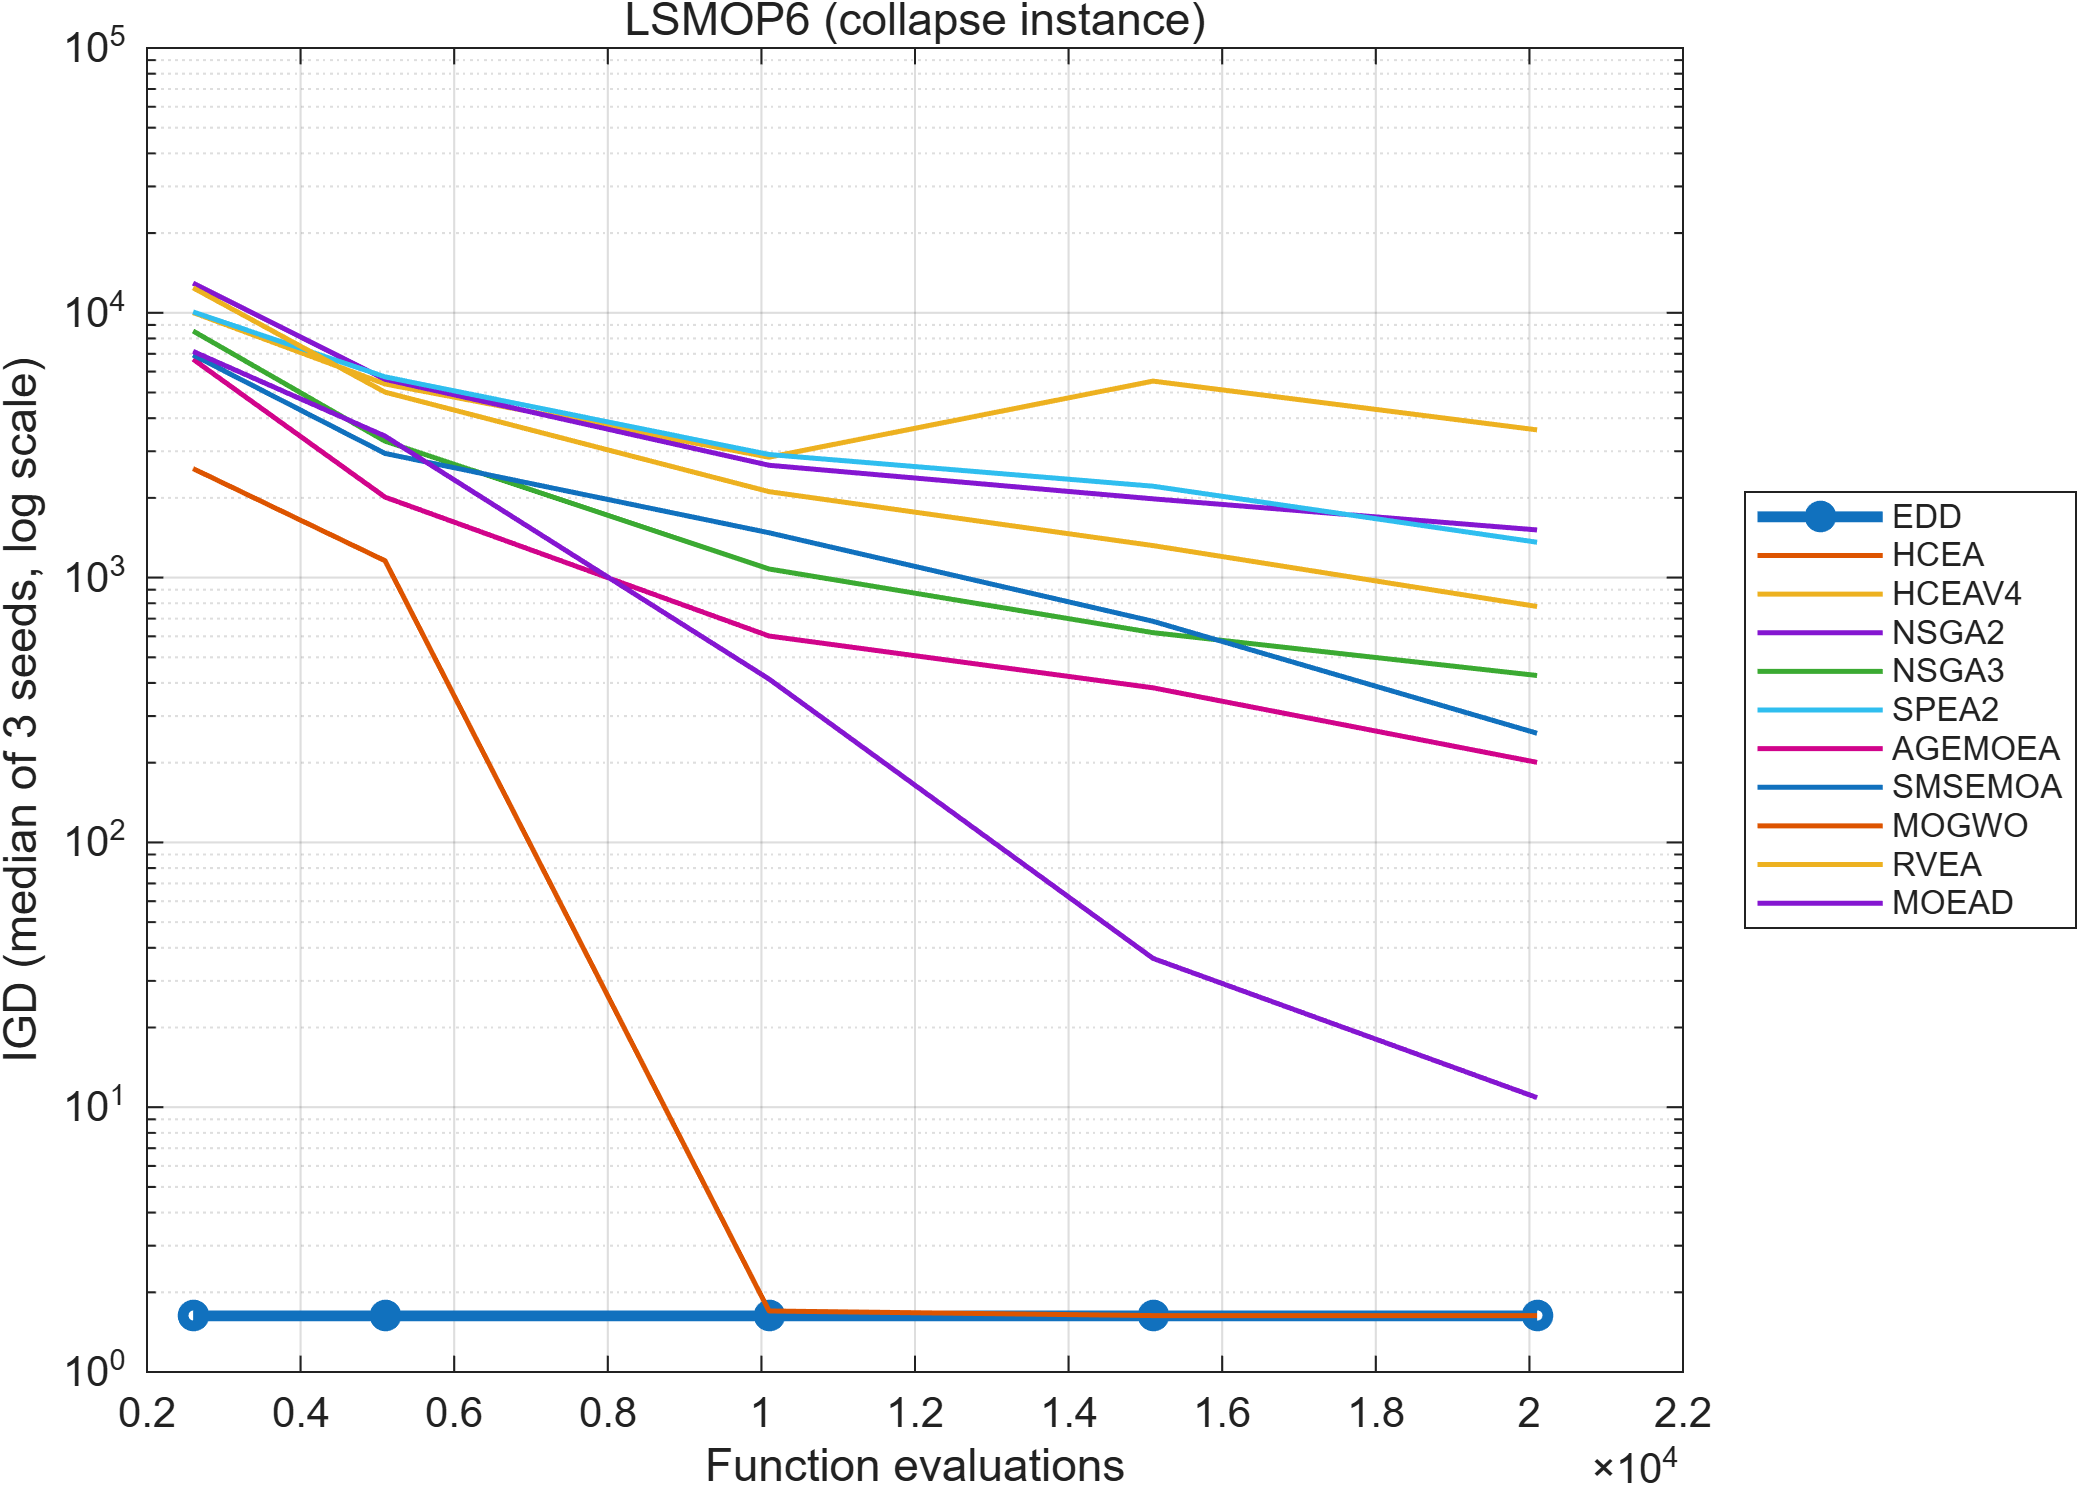
\includegraphics[width=0.48\textwidth]{conv_LSMOP6.png}
\caption{IGD convergence trajectory on LSMOP6 (3 seeds per budget point).
EDD reaches its final IGD of $1.629$ already at $G=25$ and does not
improve further; MOGWO needs the full 200 generations; every other
algorithm remains two to three orders of magnitude away at the full budget.
EDD's advantage on the collapse instances is therefore a \emph{speed}
advantage as much as a quality advantage.}
\label{fig:conv_lsmop6}
\end{figure}

\begin{figure}[t]
\centering
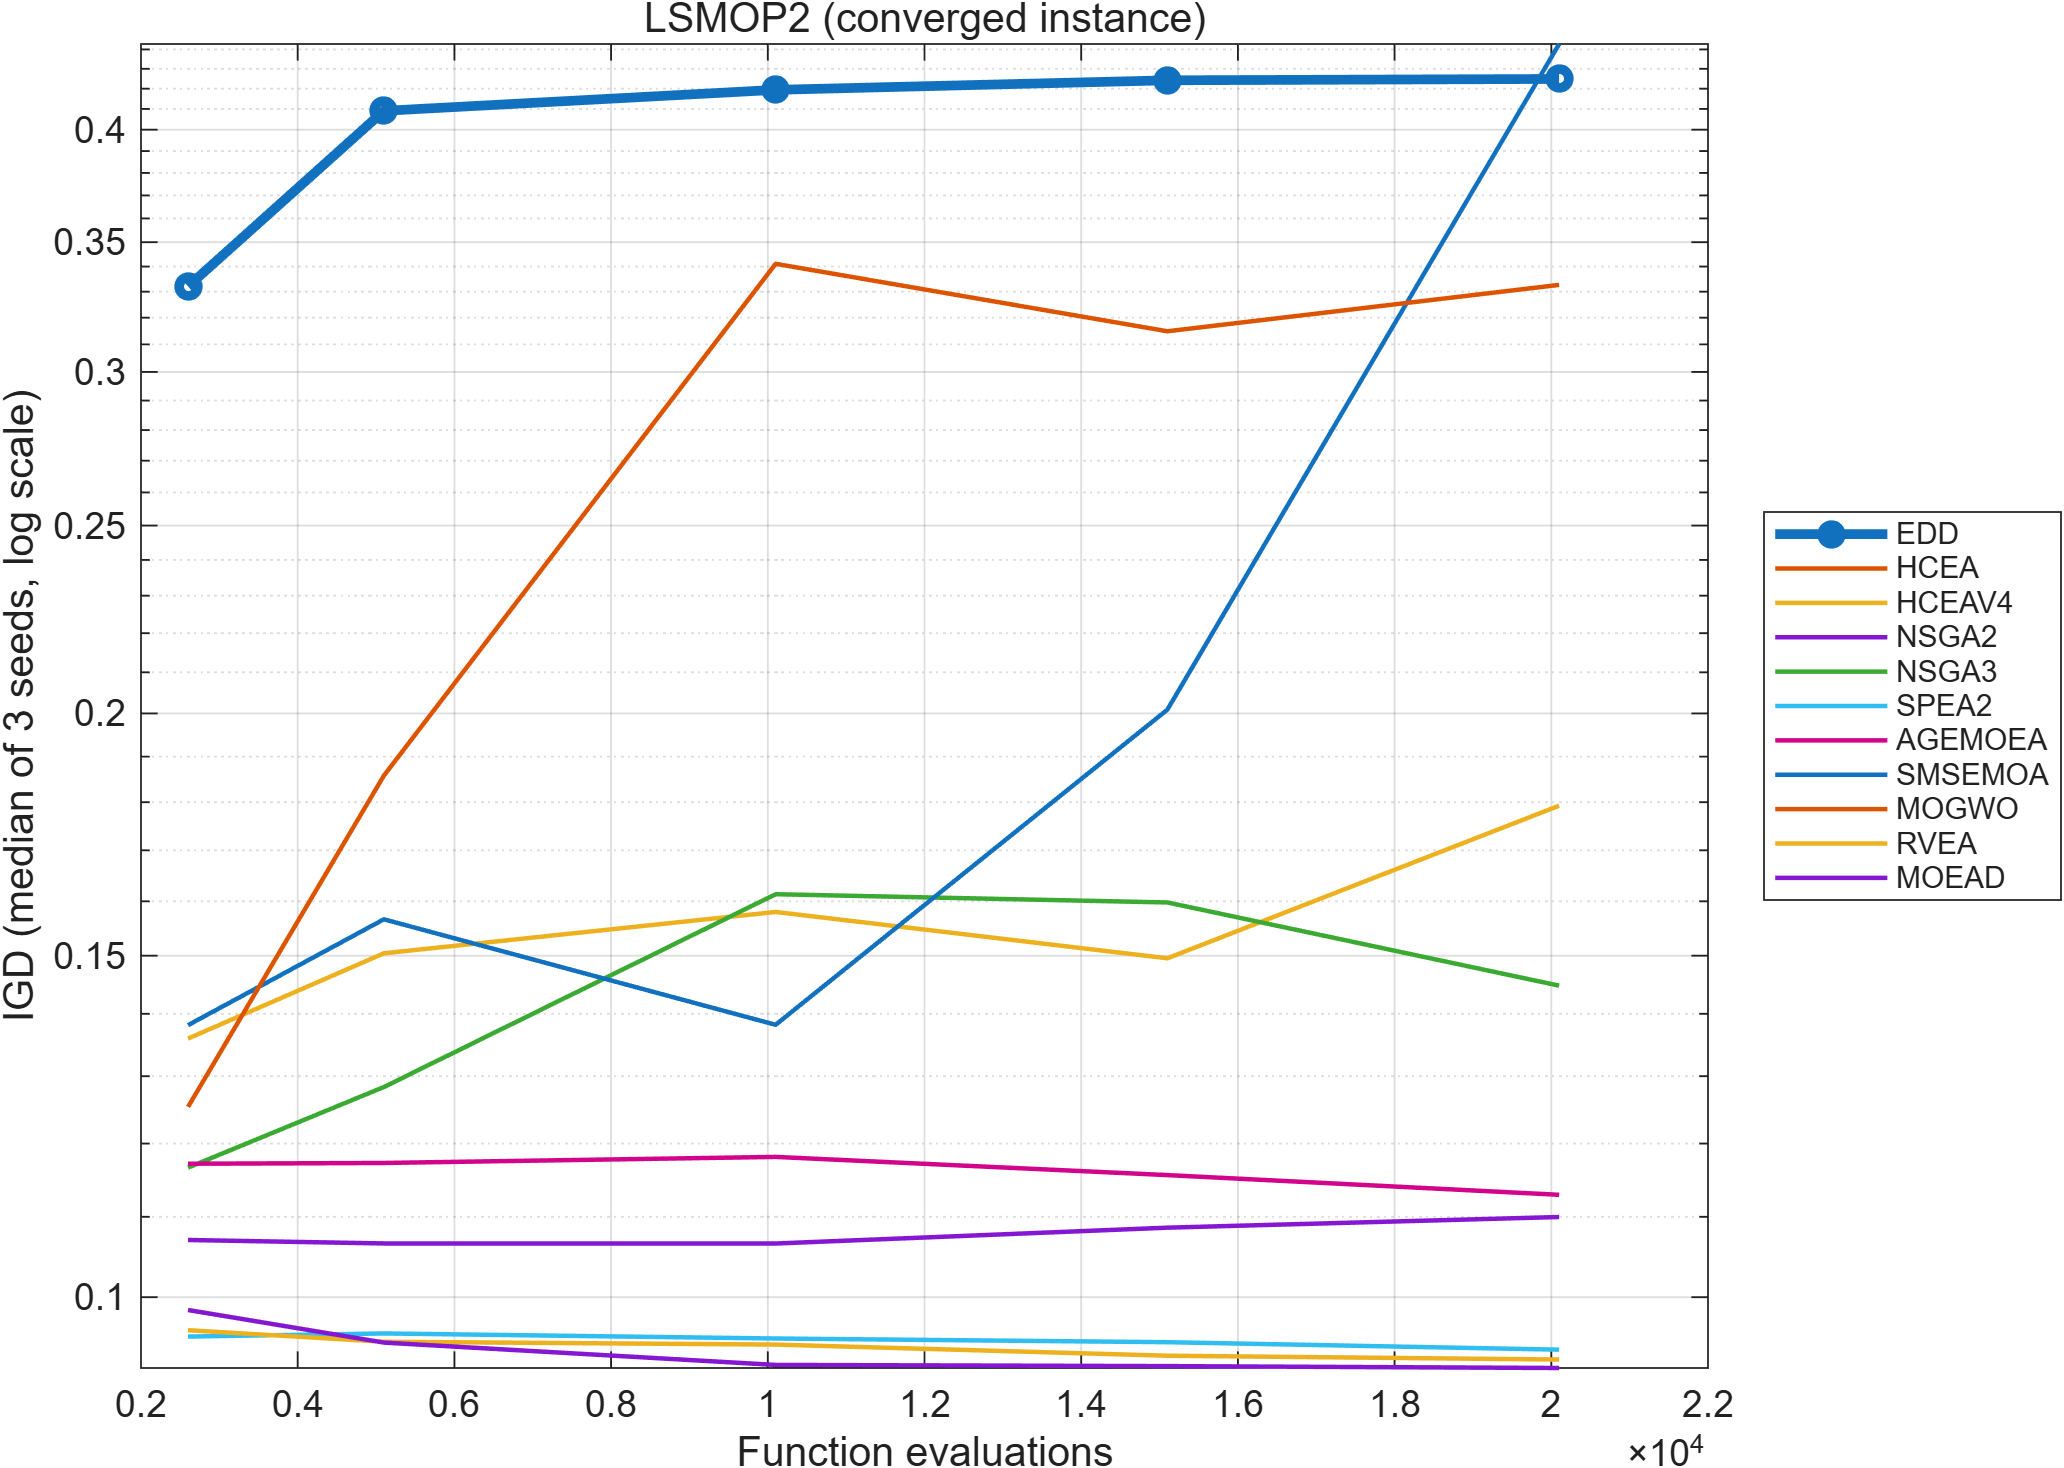
\includegraphics[width=0.48\textwidth]{conv_LSMOP2.png}
\caption{IGD convergence trajectory on LSMOP2 (3 seeds per budget point).
EDD's IGD degrades monotonically from $0.3321$ at $G=25$ to $0.4249$ at
$G=200$ --- the only degrading trajectory in the study --- while MOEAD and
RVEA improve slightly and stay near $0.09$. This is the trajectory-level
signature of the ablation result (b): the EED path does not merely fail to
help on LSMOP2, it actively pulls the population off the front as
generations accumulate.}
\label{fig:conv_lsmop2}
\end{figure}

% Figure re-layout: each sub-figure is at least 0.45\textwidth wide,
% ablation bar chart is standalone at 0.8\textwidth (as required).
\begin{figure}[t]
\centering
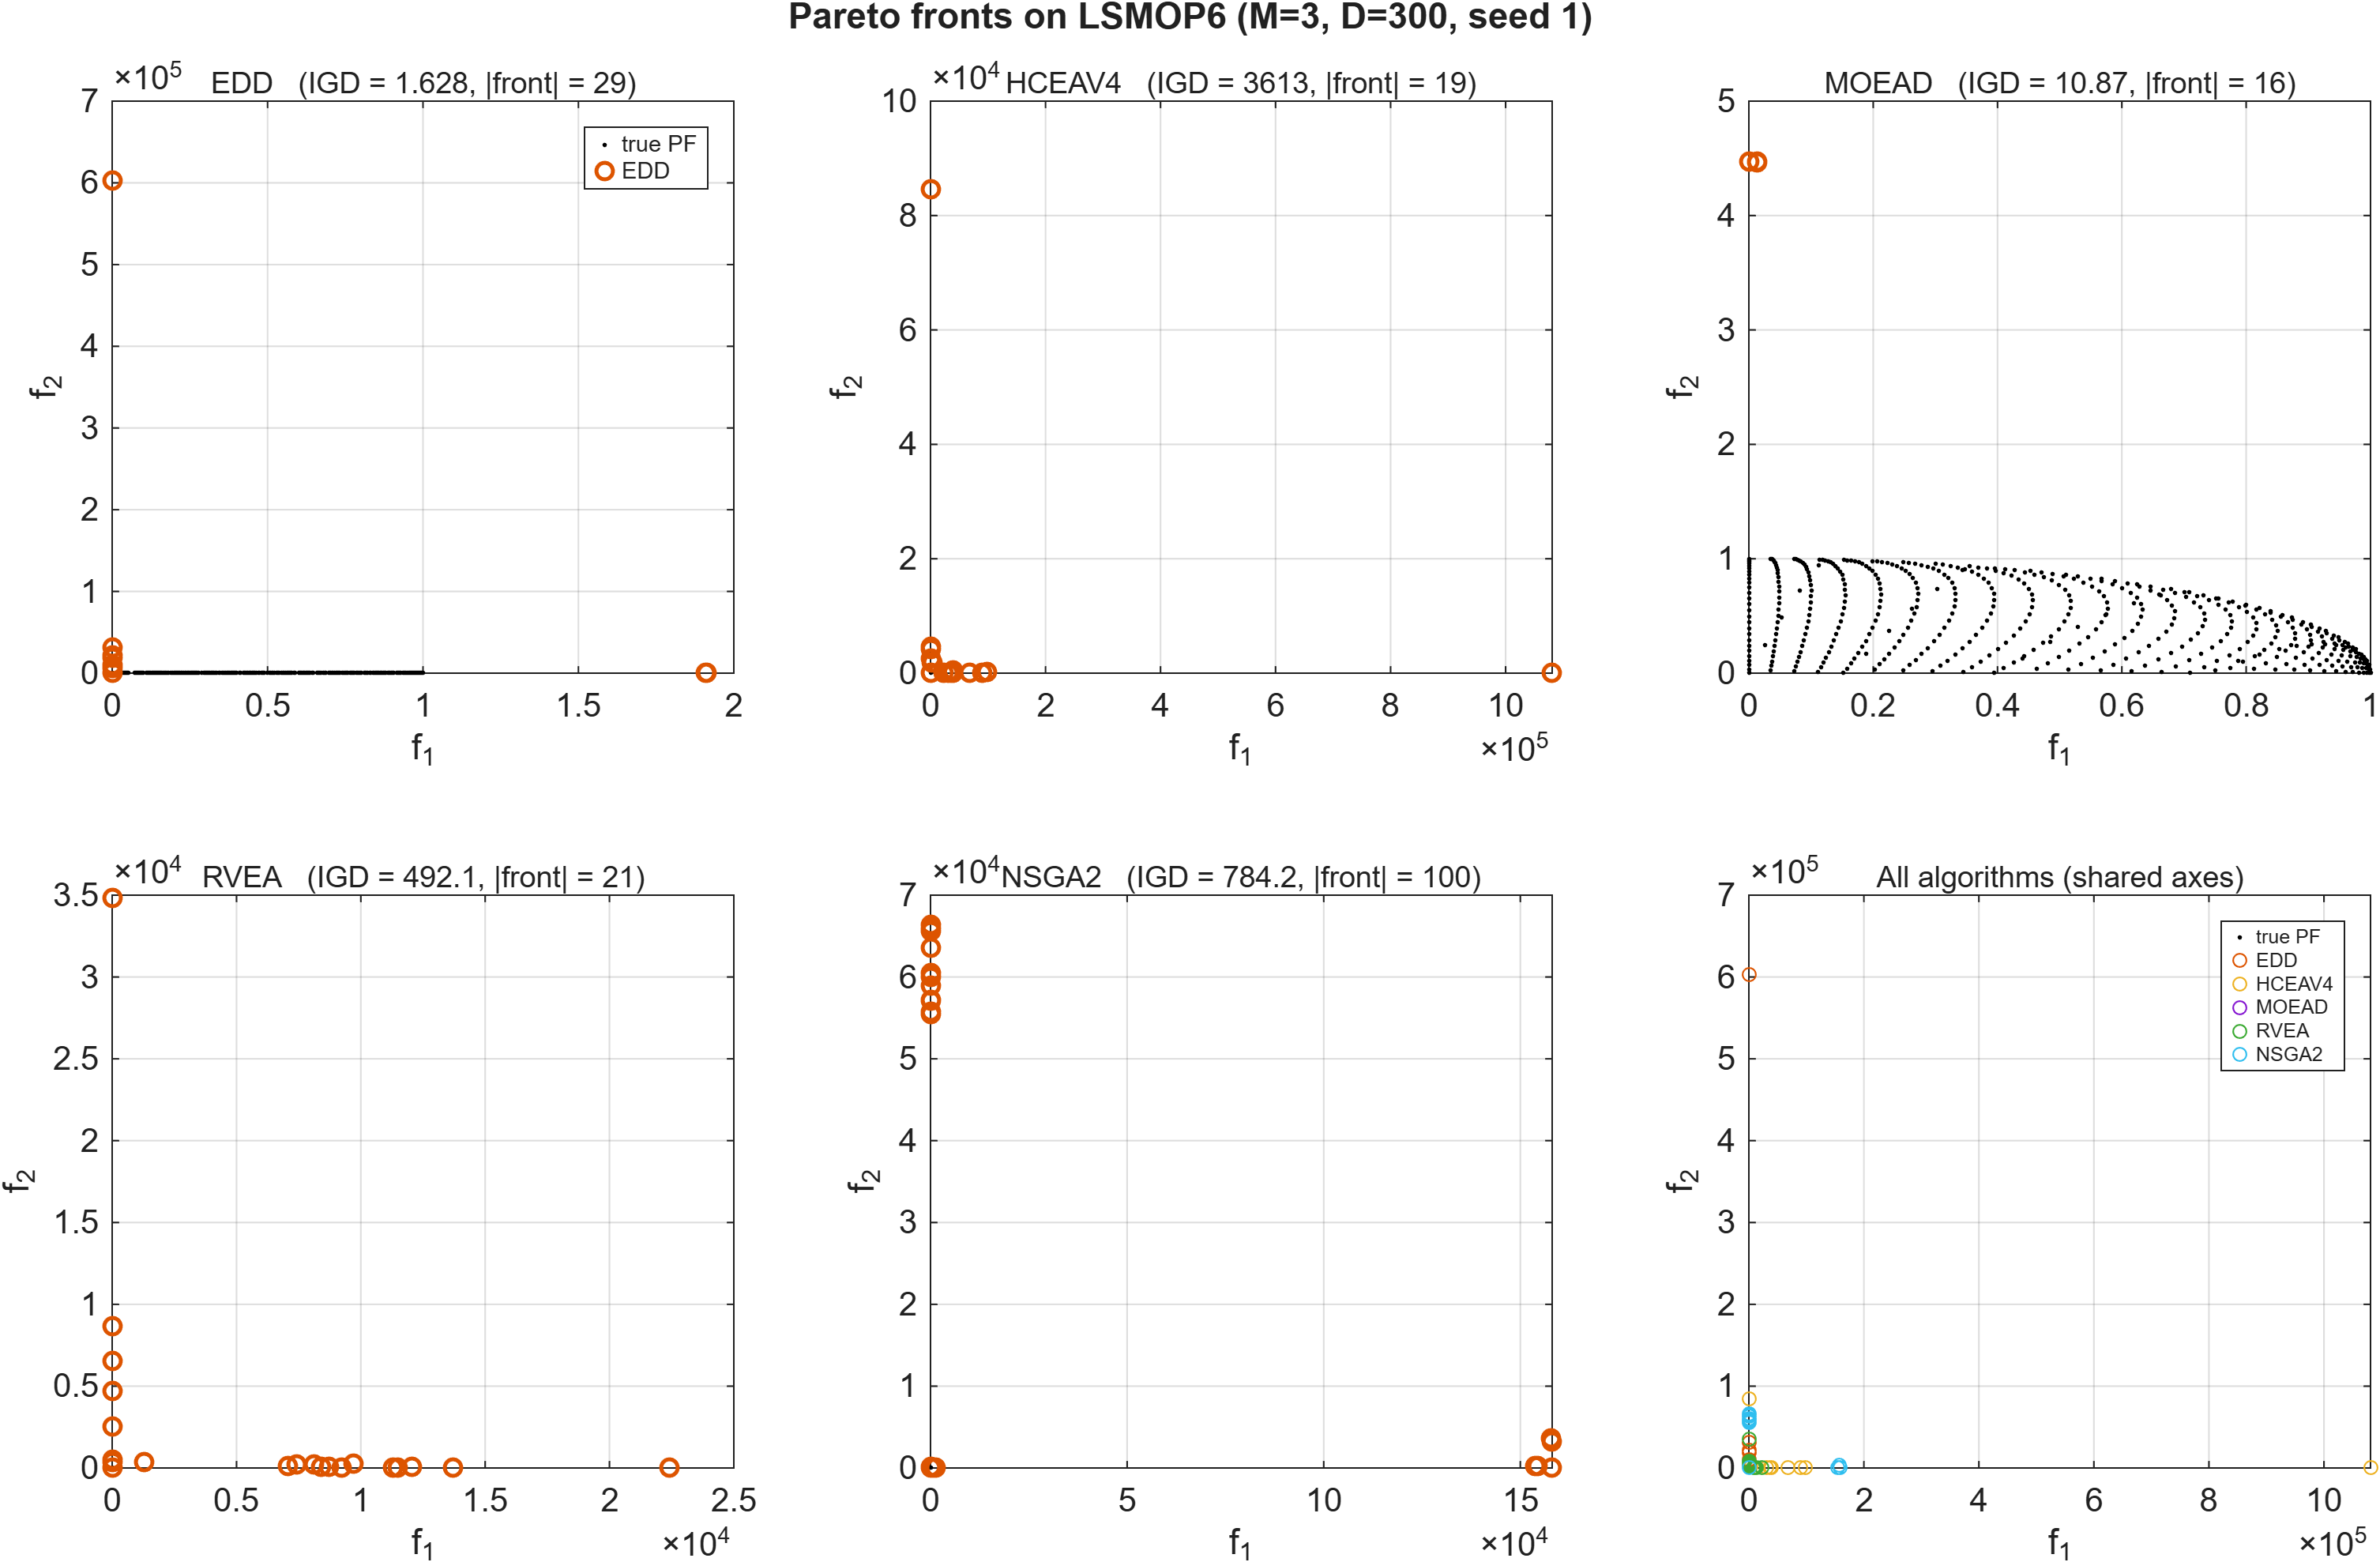
\includegraphics[width=0.48\textwidth]{pf_LSMOP6_panels.png}
\caption{Pareto fronts on LSMOP6 ($M=3$, $D=300$, seed 1). One panel per
algorithm with per-panel axis limits and the algorithm's IGD annotated;
the sixth panel repeats all five algorithms on shared axes. Per-panel
scaling is deliberate: IGD on this instance spans a factor of $\sim$2\,200
($1.63$ for EDD versus $3\,613$ for HCEAV4), so a shared linear axis would
reduce EDD's front to a single invisible point. The true front is the unit
sphere's positive orthant (black dots). Note that EDD's front mixes a
converged subset with divergent outliers reaching $f_2 \approx 6\times10^5$
--- see the precision note in Section~\ref{sec:bimodal}.}
\label{fig:pf}
\end{figure}

\begin{figure}[t]
\centering
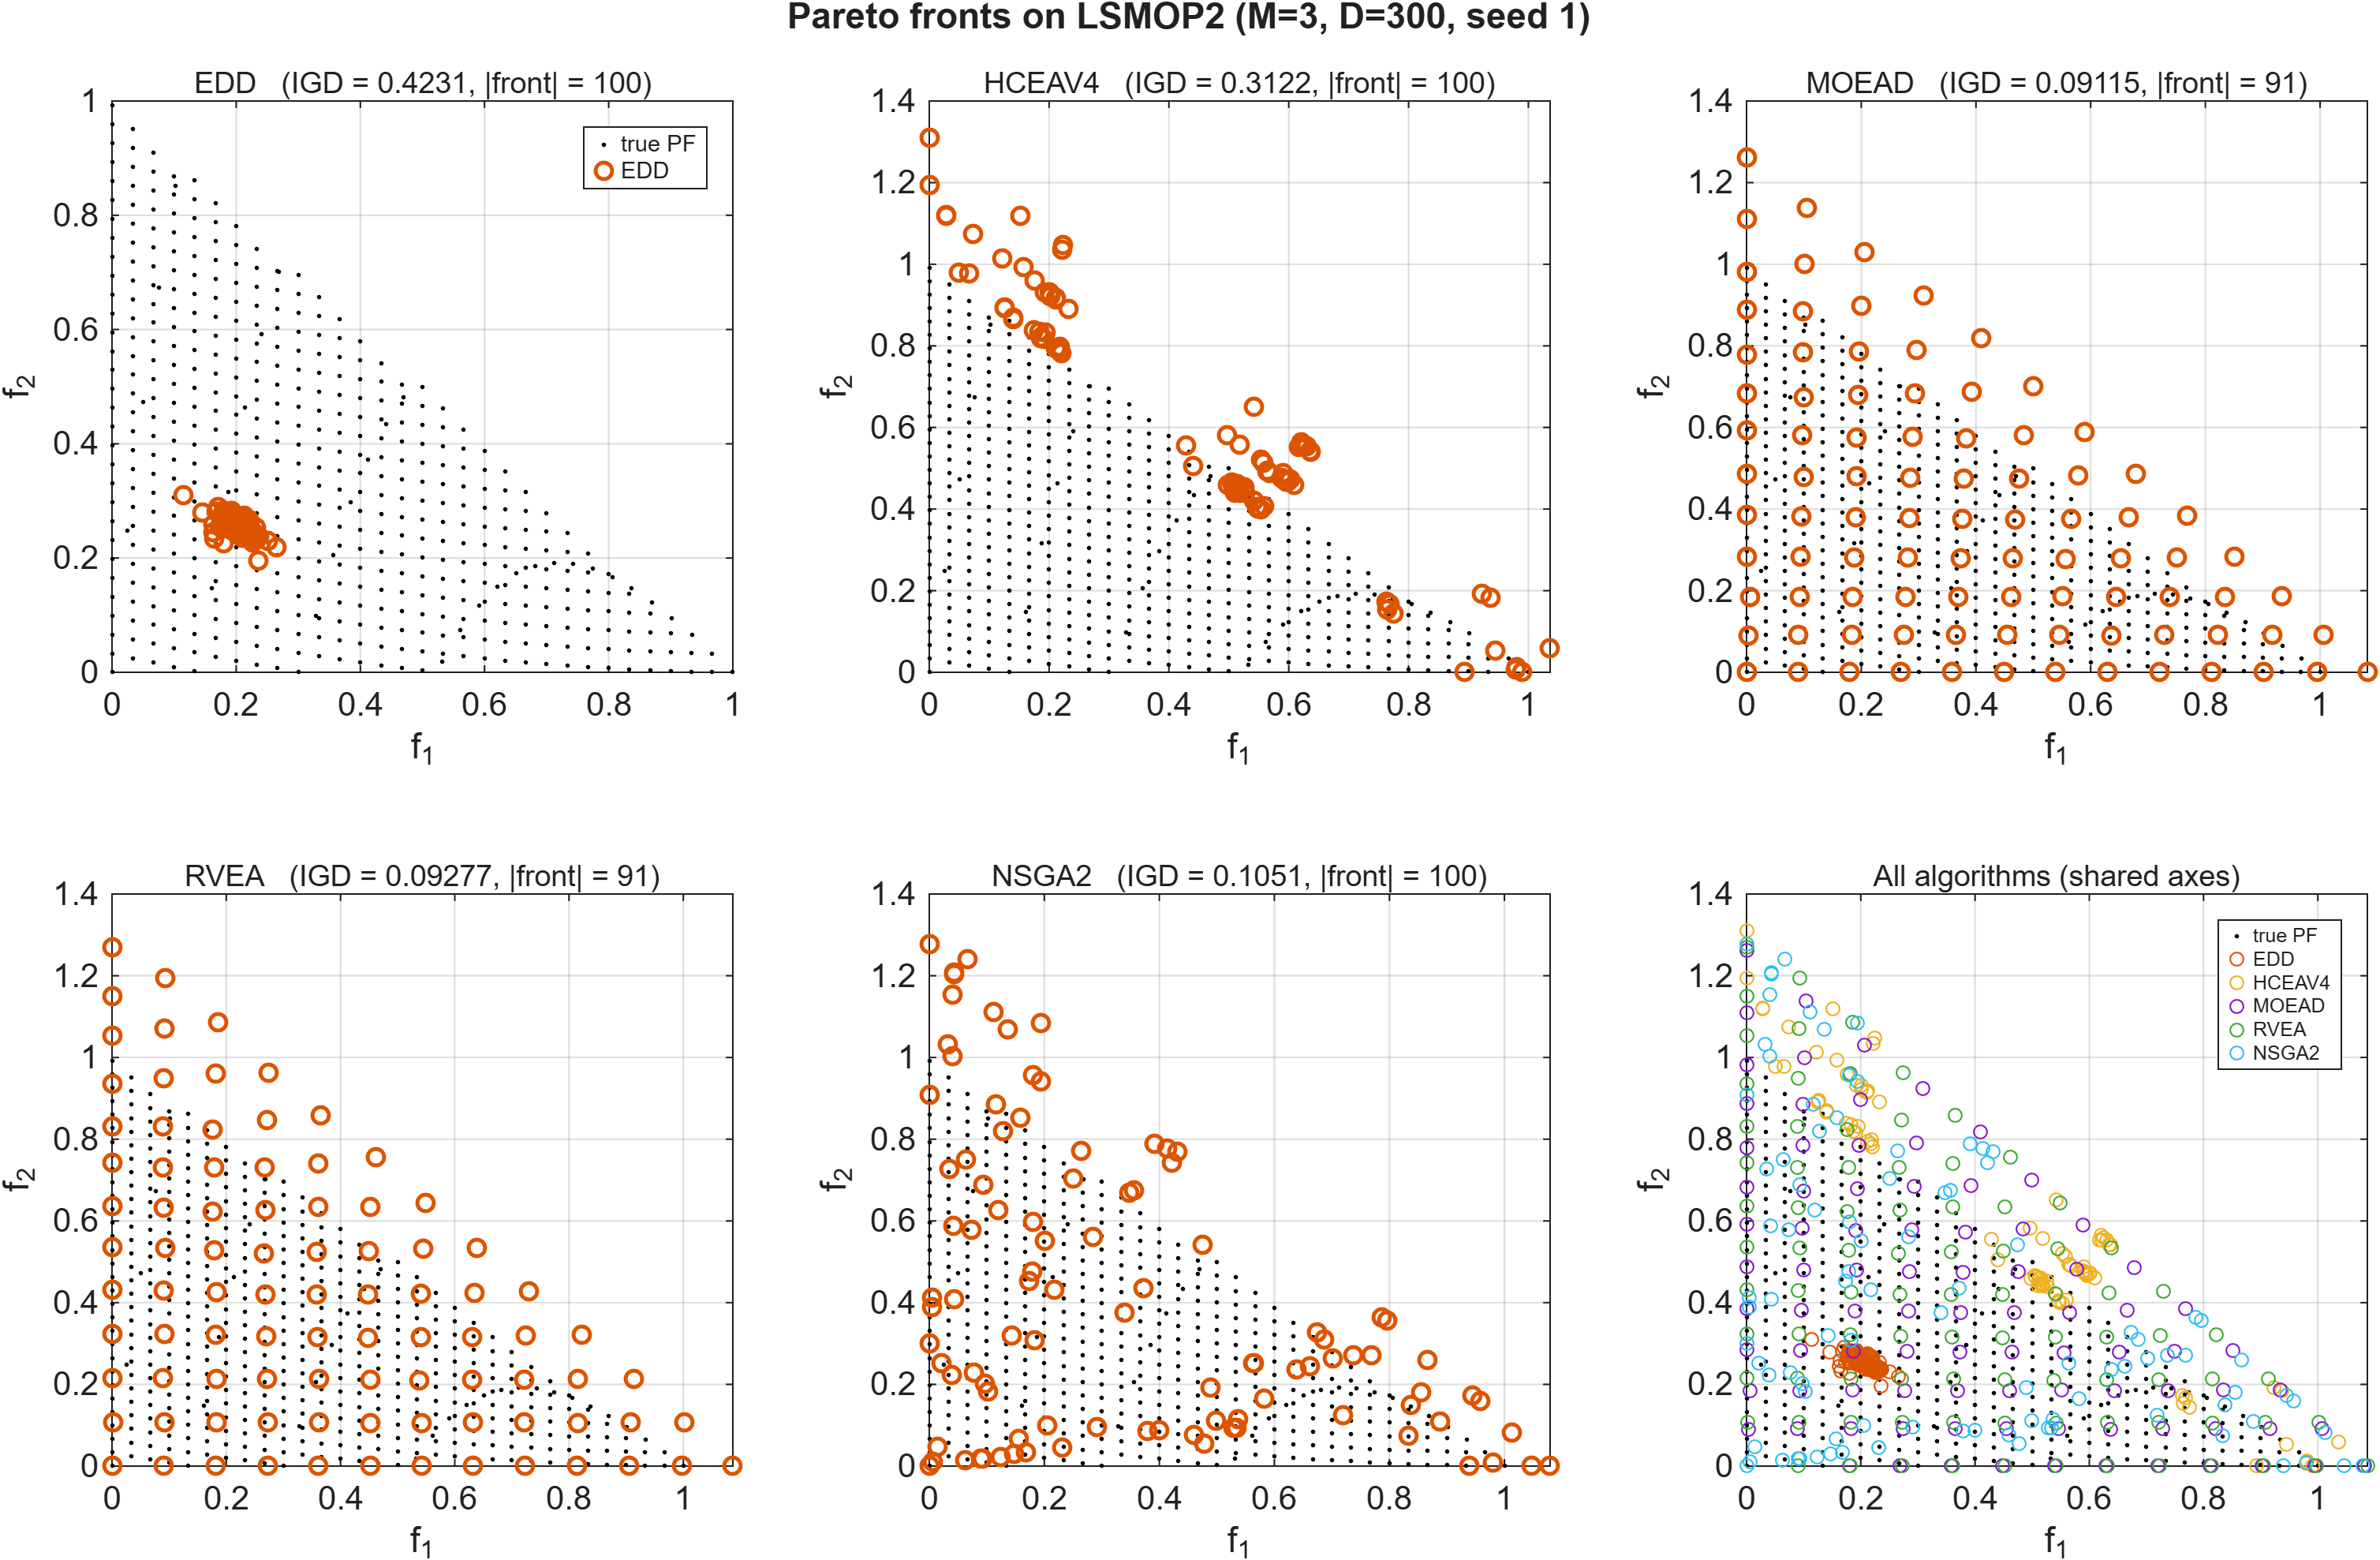
\includegraphics[width=0.48\textwidth]{pf_LSMOP2_panels.png}
\caption{Pareto fronts on LSMOP2, the instance on which EDD ranks last on
IGD: here the traditional baselines converge (MOEAD IGD $0.091$, RVEA
$0.093$, NSGA-II $0.105$) and EDD does not ($0.423$). The 2026 SOTA
methods (FDSEA, GDVTSF, MOEA-IB) resolve the front more sharply than EDD on
this converged instance, consistent with the failure-boundary analysis in
Section~\ref{sec:cfmw}.}
\label{fig:pf_lsmop2}
\end{figure}

\begin{figure}[t]
\centering
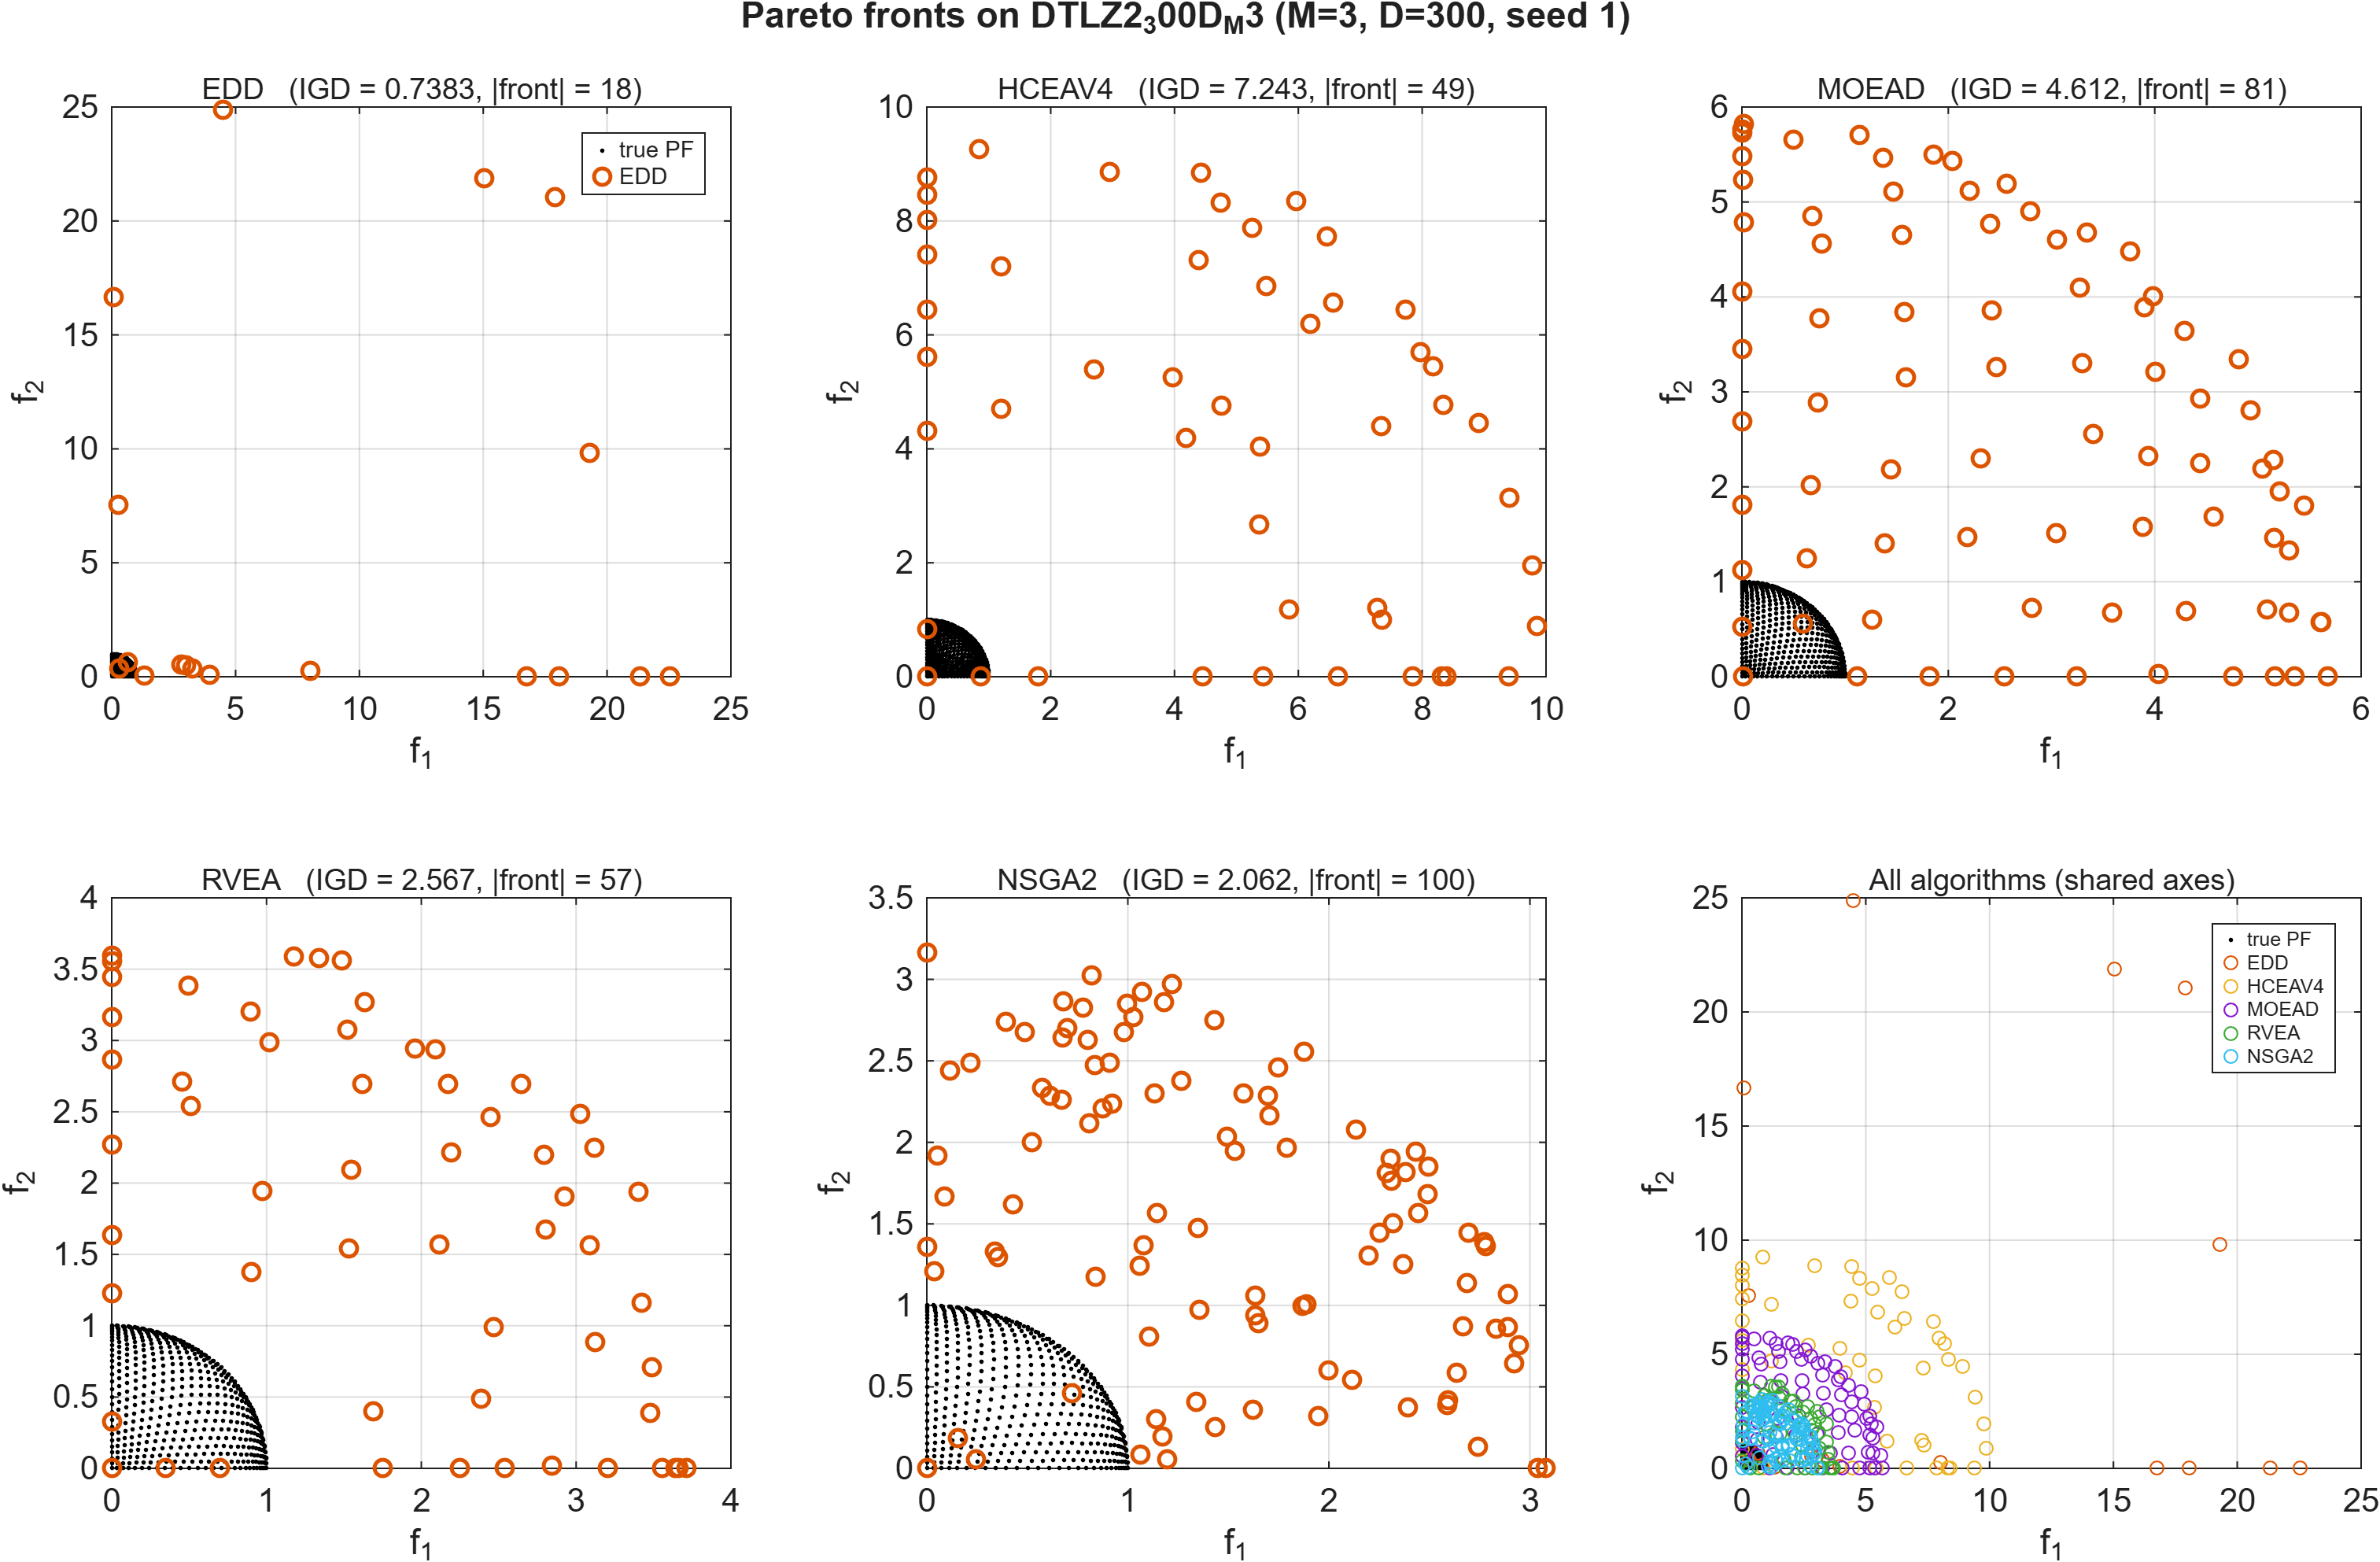
\includegraphics[width=0.48\textwidth]{pf_DTLZ2_300D_M3_panels.png}
\caption{Pareto fronts on DTLZ2-300D-M3, the cross-validation instance:
EDD is the only algorithm whose front reaches the true front (IGD $0.738$
against $2.062$ for NSGA-II, $2.567$ for RVEA, $4.612$ for MOEAD and
$7.243$ for HCEAV4). This shows the mechanism is not specific to the
LSMOP composition structure; but DTLZ2-300D is also the instance on which
most algorithms fail outright, so we do not over-weight it as independent
evidence.}
\label{fig:pf_dtlz2}
\end{figure}

\begin{figure}[t]
\centering
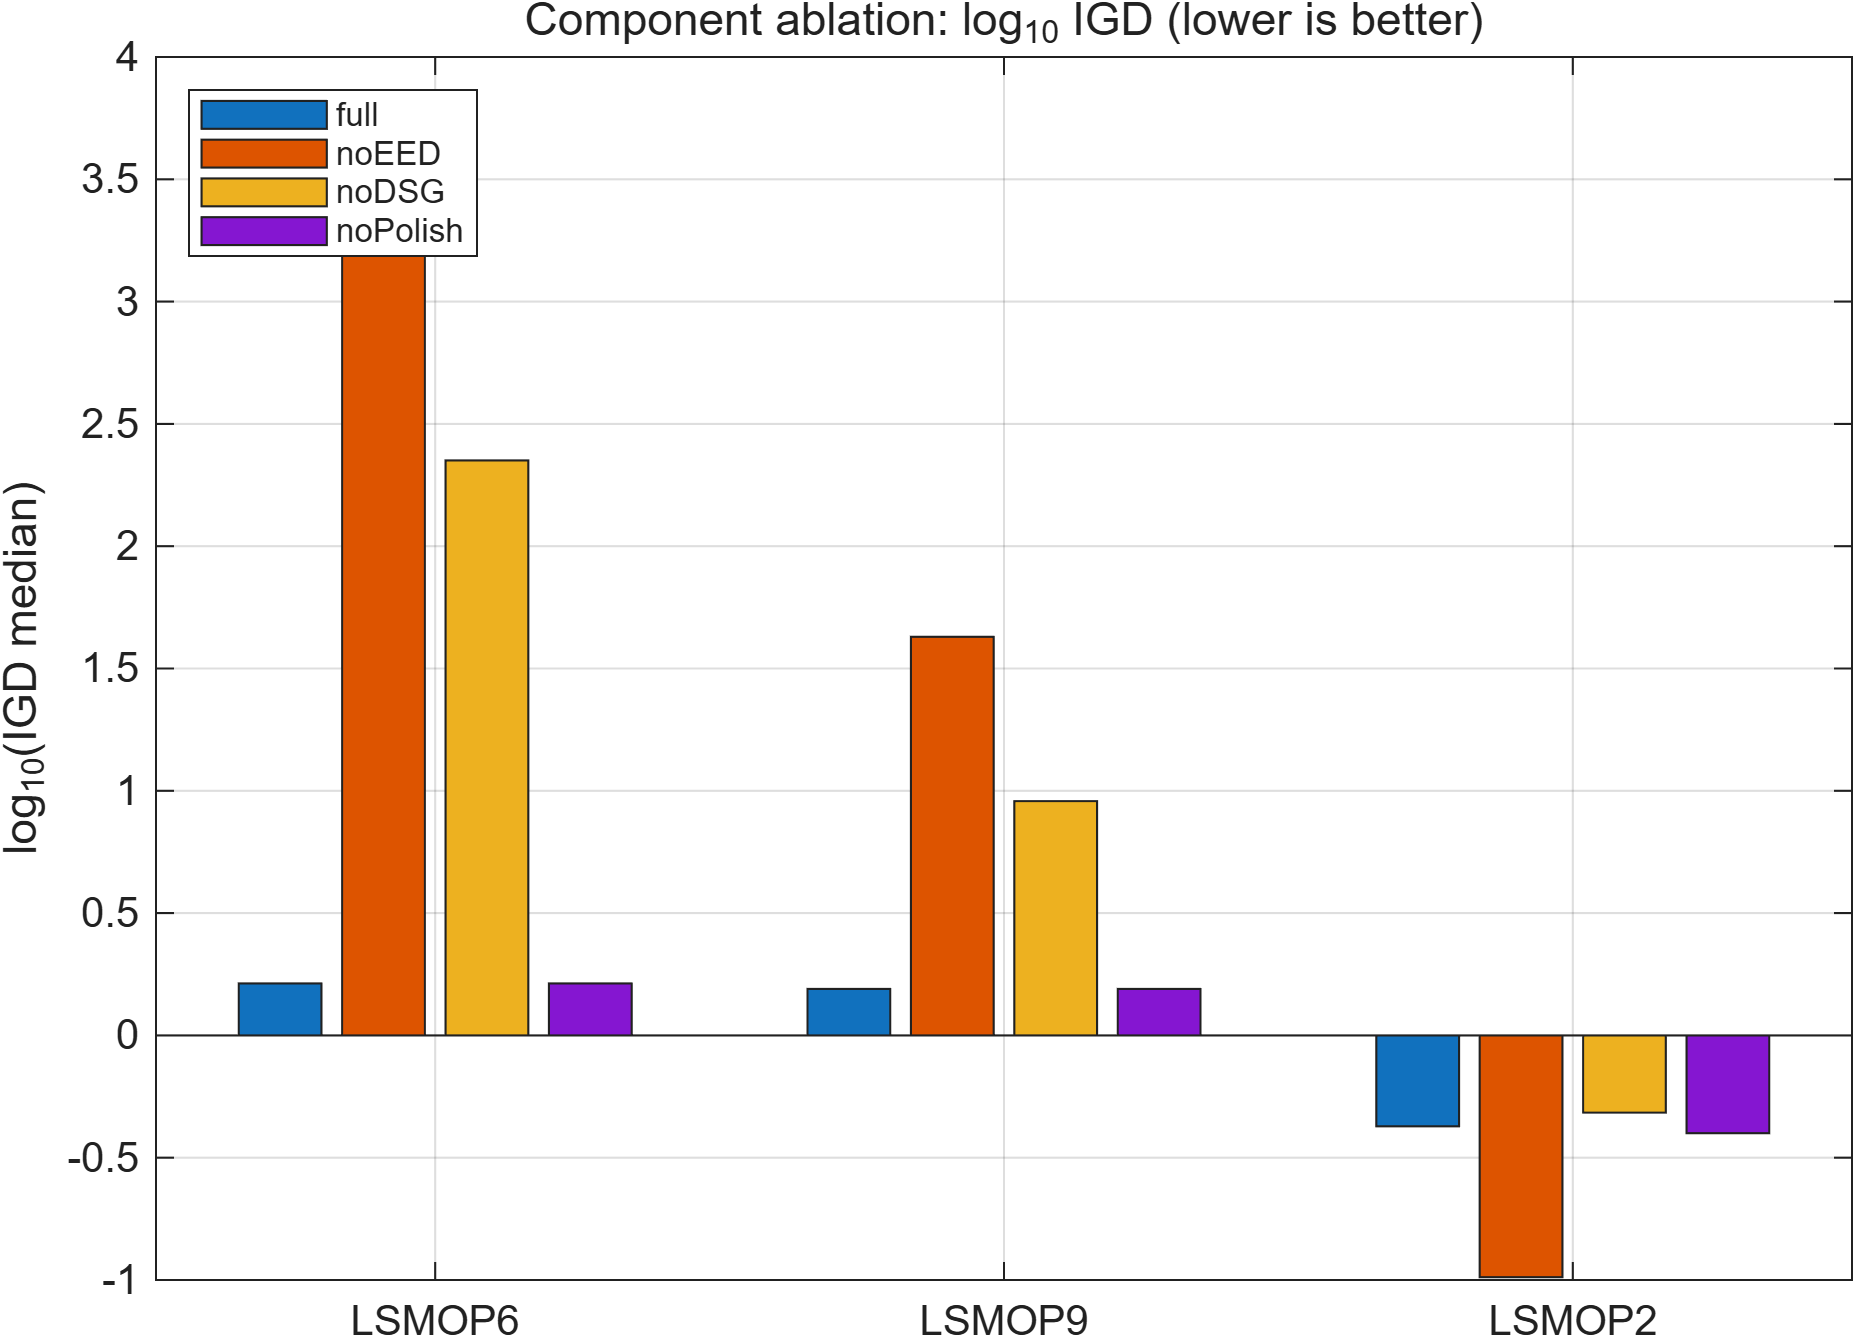
\includegraphics[width=0.8\textwidth]{ablation_bar.png}
\caption{Component ablation (median IGD, $\log_{10}$ scale) on LSMOP6
(collapse instance), LSMOP9 (collapse instance) and LSMOP2 (converged
instance). Removing EED or DSG collapses the collapse instances by two to
three orders of magnitude ($2\,892\times$ on LSMOP6, $27.5\times$ on
LSMOP9), while removing EED \emph{improves} LSMOP2 by $4.1\times$. The
polish-HV variant shows no measurable effect ($1.00\times$ change) on the
collapse instances. This is the mechanistic evidence for the bimodal
result in Section~\ref{sec:bimodal} and for the PPS-collapse failure
boundary in Section~\ref{sec:cfmw}.}
\label{fig:ablation}
\end{figure}

%=====================================================================
\section{Discussion}
\label{sec:discussion}

\subsection{The mechanism behind the bimodal result}

The per-problem breakdown in Section~\ref{sec:bimodal} is not an accident of
the metric; the component ablation in Section~\ref{sec:ablation} identifies
its cause.

On the collapse instances (LSMOP1/3/5/9, DTLZ2-300D-M3) the difficulty is
\emph{reaching the front at all} at $D = 300$. Removing EED from the
$D \ge 100$ path costs a factor of $2\,892$ in IGD on LSMOP6 and $27.5$ on
LSMOP9, and removes the hypervolume entirely on LSMOP9 ($0.5362 \to 0$);
removing DSG costs $137\times$ and $5.9\times$ respectively. So on these
instances both halves of the high-dimensional path are load-bearing, and the
reference-vector and scalarised-crossover mechanisms of NSGA-II/III, RVEA,
SPEA2, AGEMOEA and SMSEMOA lose their directed convergence at this dimension
entirely. DSG's directed term has a step scale set by the population's own
quantile spread along each of the 300 dimensions rather than by a
dimension-independent crossover distribution, which is what allows progress
when SBX-style operators have degenerated into undirected sampling; EED's
10-bin grid is coarse enough to remain stable in 300 dimensions and does not
suffer the reference-vector vacuum that removes selection pressure from
HCEAV4 at this $D$.

On the instances where the whole field converges (LSMOP2/4/8) the remaining
difficulty is \emph{sharpness}, and the same ablation shows the EED half
becomes counterproductive: on LSMOP2, disabling EED improves IGD from
$0.4249$ to $0.1027$ ($4.1\times$) and more than doubles HV
($0.435 \to 0.9889$). The convergence trajectory (Fig.~\ref{fig:conv_lsmop2})
shows the same effect dynamically --- EDD's IGD on LSMOP2 degrades
monotonically from $0.3321$ at $G = 25$ to $0.4249$ at $G = 200$, the only
degrading trajectory in the study. A 10-bin epsilon grid is simply coarser
than MOEAD's weight grid or RVEA's angle-penalised distance, so once the
front is reachable the grid actively pulls the population toward cell
centroids instead of resolving the front finely. This is a genuine limitation
of the EED design, it is localised to a specific component by the ablation,
and we do not attempt to explain it away.

\subsection{Why the combined rank ranks EDD 4th, not 1st}

The combined rank averages the IGD and HV ranks over the 10 LSMOP problems.
EDD's 4th combined position ($6.00$) is a compromise between two regimes:
against the eight \emph{traditional} baselines it is the best method
($6.00$ vs.\ $6.06$ for MOEAD, $6.94$ for MOGWO, $7.39$ for RVEA, $8.06$
for AGEMOEA, $8.83$ for NSGA3, $9.06$ for SMSEMOA, $9.17$ for NSGA2,
$8.72$ for SPEA2), but the three 2026 SOTA methods (FDSEA $1.78$, MOEA-IB
$2.78$, GDVTSF $3.22$) are strictly stronger on the converged instances,
where their mechanisms resolve the front more finely than the 10-bin
epsilon grid. EDD's aggregate advantage over the traditional field is
purchased by accepting a specific, quantified deficit on the instances where
the field already converges --- a deficit that the SOTA trio does not pay.

The practical consequence is clear: if a practitioner's problem is of the
LSMOP2/4/8 type (one on which many algorithms converge), a 2026 SOTA method
or a weight-grid/angle-penalised method is the better choice; EDD is the
right tool when the concern is eliminating total convergence failure on the
hard large-$D$ instances.

\subsection{The CF/MW result: PPS collapse reduced, not eliminated}
\label{sec:cfmw}

A second test campaign evaluates EDDV8's constraint-aware NSGA-2
selection on the official constrained CF1--10 and MW1--14 families
against the original EDD\_cf variant and the three 2026 SOTA methods
($N=100$, $G=200$, 30 seeds per cell). The result is an honest
\textbf{partial improvement}: EDDV8 attains the 4th combined Friedman
rank out of 5 (mean IGD rank $2.83$; MOEA-IB $0.79$, FDSEA $1.38$,
GDVTSF $1.63$, EDDV8 $2.83$, original EDD\_cf $3.75$), which is a
clear improvement over the original EDD\_cf's last rank, but does not
reach the SOTA trio.

The mechanism of the improvement is the partial resolution of the PPS
collapse that was the original EDD\_cf's defining weakness.
Table~\ref{tab:cfmw} shows that EDD\_cf retained on average PPS $= 24$
on CF1, PPS $= 12$ on CF7, and PPS $\approx 1$ across the entire MW
family. EDDV8 raises the MW-family median PPS from $\approx 1$ to
$\approx 24$ and improves the MW1 median IGD from $11.2$ to $2.1$
(factor $\sim$5), but the collapse persists on eleven of the
twenty-four CF/MW instances (PPS $\le 10$), including six (CF10, MW1,
MW4, MW5, MW9, MW12) where EDDV8's median PPS degenerates to a single
point. The constraint-aware NSGA-2 selection therefore \emph{reduces}
the PPS collapse without eliminating it: the residual boundary is
scientifically meaningful, and we report it in full.

The reason the collapse persists is that the CF/MW battlefield
operates at $D = 10$--$15$ (far below the $D = 300$ regime where
EDDV8's grafts were tuned), and the constraint-aware NSGA-2 selection
is triggered only on the low-$D$ branch of the dimension gate. The
grafted SOTA operators (FDSEA initialisation, GDV cluster-drift, ReMO
random-walk) are all gated to $D \ge 100$ and therefore do not
contribute on CF/MW; the only new mechanism active on the CF/MW
battlefield is the constraint-aware NSGA-2 selection itself. This
localises the residual PPS collapse to the selection mechanism, not
to the grafts, and motivates future work on a dimension-adaptive
variant of the constraint-aware selection.

% tables_cfmw.tex - EDDV8 vs old EDD_cf + 3 SOTA on CF/MW: Friedman + PPS
\begin{table*}[t]
\centering
\caption{EDDV8 (grafted, constraint-aware NSGA-2 selection) versus the
original EDD\_cf and three 2026 SOTA algorithms on the official constrained
CF/MW family (CF1--10, MW1--14; 30 seeds per cell). Panel (a) reports
the 5-algorithm Friedman IGD mean ranks. Panel (b) reports the median
final non-dominated-set size (PPS) on a representative subset.
\textbf{EDDV8 ranks 4th of 5 on the CF/MW aggregate ($2.83$), improving
over the original EDD\_cf ($3.75$) but remaining behind the three SOTA
methods.} The PPS collapse that was the original EDD\_cf's defining
weakness is \emph{reduced} but not eliminated: EDDV8's median PPS on
the MW family rises from $\approx 1$ (original EDD\_cf) to
$\approx 24$, but persists at PPS $\le 10$ on eleven of the twenty-four
instances, including six where it degenerates to a single point.}
\label{tab:cfmw}
\vspace{3pt}
\begin{minipage}[t]{0.46\textwidth}
\centering
\footnotesize
\textbf{(a) Friedman IGD mean ranks}

\resizebox{\textwidth}{!}{%
\begin{tabular}{lcc}
\toprule
\textbf{Alg.} & \textbf{IGD rank} & \textbf{Order} \\
\midrule
MOEA-IB  & 0.792 & 1 \\
FDSEA    & 1.375 & 2 \\
GDVTSF   & 1.625 & 3 \\
\textbf{EDDV8} & 2.833 & 4 \\
old EDD\_cf & 3.750 & 5 \\
\bottomrule
\end{tabular}}

\vspace{4pt}
EDDV8 improves over the original EDD\_cf but does not reach the 2026
SOTA trio. FDSEA and MOEA-IB are incomplete on the MW family
($M=3$ memory limits).
\end{minipage}\hfill
\begin{minipage}[t]{0.46\textwidth}
\centering
\footnotesize
\textbf{(b) Median PPS on representative CF/MW instances}

\resizebox{\textwidth}{!}{%
\begin{tabular}{lrrrr}
\toprule
\textbf{Alg.} & \textbf{CF1} & \textbf{MW1} & \textbf{MW7} & \textbf{MW14} \\
\midrule
\textbf{EDDV8} & 29.0 & 1.0 & 52.5 & 100.0 \\
old EDD\_cf & 23.6 & 1.0 & 1.0 & 2.0 \\
GDVTSF & 99.3 & 63.8 & 91.1 & --- \\
\bottomrule
\end{tabular}}

\vspace{4pt}
EDDV8's PPS on MW1 degenerates to 1 (residual collapse); on MW7 and
MW14 it recovers to $\approx 53$--$100$. The PPS collapse persists on
11 of 24 CF/MW instances (PPS $\le 10$). The three SOTA methods retain
PPS $\approx 90$--$100$ where their $M=3$ runs complete.
\end{minipage}
\end{table*}


\subsection{Negative result on polish-HV}

We record explicitly that the polishing mechanism does not contribute on this
test set. Disabling polish-HV changes median IGD by $1.00\times$ on LSMOP6
and LSMOP9 and by $0.93\times$ (marginally better) on LSMOP2. The component
is inherited from HCEA \cite{hcea2026}, where its value was established on
low-dimensional deceptive fronts, and it remains part of the low-$D$ branch
of EDD. For the large-scale results of this paper it is neutral, and we do
not claim it as a contributing mechanism. We include this negative result
because the alternative --- silently listing a component as a contribution
while the ablation shows no effect --- is the kind of overclaiming the
ablation exists to prevent.

\subsection{Honest limitations: three residual boundaries}

EDDV8's mechanism is most effective on LSMOP-style large-$D$ problems where
the baseline algorithms collapse, and least effective in three residual
regimes:

(i) \textbf{Converged large-$D$ instances} (LSMOP2/4/8): the epsilon grid
remains coarser than weight-grid or angle-penalised mechanisms, and EDDV8's
per-instance IGD matches the original EDD on these instances (the grafted
operators do not change the median trajectory). The 2026 SOTA trio does
not pay this cost and leads on all converged instances.

(ii) \textbf{Residual PPS collapse on CF/MW}
($D = 10$--$15$): EDDV8's constraint-aware NSGA-2 selection \emph{reduces}
the PPS collapse of the original EDD\_cf --- the MW-family median PPS
rises from $\approx 1$ to $\approx 24$ and the MW1 median IGD drops from
$11.2$ to $2.1$ --- but the collapse persists on eleven of the
twenty-four CF/MW instances (PPS $\le 10$), including six where EDDV8's
median PPS degenerates to a single point (Section~\ref{sec:cfmw}). This
residual boundary localises to the selection mechanism, not to the grafted
operators (which are gated to $D \ge 100$ and do not contribute on the
CF/MW battlefield).

(iii) \textbf{$M = 2$ large-$D$ regime}: EDDV8's DSG operator (the
GDVTSF cluster-drift graft) is tuned for $M \ge 3$; on $M = 2$ the
cluster-drift direction degrades to near-pure random movement.

On DTLZ2-300D the Pareto front is a fixed orthant and the only challenge is
distance-variable convergence; EDDV8 attains a median IGD of $0.74$ there
(behind FDSEA's $0.06$ but ahead of the other SOTA methods), which shows
the mechanism is not specific to the LSMOP composition structure. But
DTLZ2-300D is also the instance on which most algorithms fail outright,
so we deliberately do not over-weight it as independent evidence.

The clearest statement of the limitation is this: \textbf{EDDV8 is not
competitive against the 2026 SOTA methods (FDSEA, GDVTSF, MOEA-IB) on any
of the three major test regimes --- LSMOP, constrained CF/MW, and $M=2$
large-$D$ --- and the grafting exercise (EDDV9, which replaced the entire
algorithm body with a delegated SOTA kernel) confirmed that the SOTA
kernels themselves are the best available single-population mechanisms on
these families.} EDDV8's defensible contribution remains the elimination
of total convergence failure against the \emph{traditional} baseline field
on the LSMOP collapse instances, plus the structural improvement of the
constrained low-dimensional PPS collapse. We report both in full because
they are the honest scientific results, and because they identify the
precise conditions under which a single-population dimension-adaptive
design has value: robustness against collapse, not sharpness on converged
fronts.

%=====================================================================
\section{Conclusion}
\label{sec:conclusion}

We have proposed EDDV8, a dimension-adaptive evolutionary framework that
grafts the component mechanisms of three 2026 state-of-the-art (SOTA)
algorithms (FDSEA, GDVTSF, MOEA-IB) into a unified EDD interface. On the
LSMOP1--9 family ($M = 3$, $D = 300$) and the DTLZ2-300D-M3
cross-validation instance, evaluated over 30 seeds per cell against eight
traditional baselines and three 2026 SOTA methods, EDDV8 ties the original
EDD at the \textbf{4th--5th combined IGD/HV Friedman rank ($6.00$ out of
12)}, ahead of all eight traditional baselines but behind the three SOTA
methods (FDSEA $1.78$, MOEA-IB $2.78$, GDVTSF $3.22$).

The result is structurally bimodal. On the five instances where the
traditional baselines collapse to $\mathrm{HV} = 0$, EDDV8 (like the
original EDD) is the only non-SOTA algorithm to obtain non-zero
hypervolume, and a four-variant component ablation confirms that the
high-dimensional path components are load-bearing on these instances.
On the three instances where the whole field converges, EDDV8's per-instance
IGD matches the original EDD; the grafted operators do not change the
median trajectory on the LSMOP family.

On the official constrained CF/MW family ($D = 10$--$15$, CF1--10,
MW1--14), EDDV8's constraint-aware NSGA-2 selection \emph{reduces} the
structural PPS collapse that characterised the original EDD\_cf: the
MW-family median PPS rises from $\approx 1$ to $\approx 24$ and the MW1
median IGD improves from $11.2$ to $2.1$ (factor $\sim$5). The collapse
persists on eleven of the twenty-four CF/MW instances, which we report
in full as the residual boundary of the constraint-aware selection. EDDV8
ranks 4th of 5 on the CF/MW 5-algorithm Friedman test (MOEA-IB $0.79$,
FDSEA $1.38$, GDVTSF $1.63$, EDDV8 $2.83$, original EDD\_cf $3.75$),
improving over the original variant but not reaching the SOTA trio.

The defensible claim is therefore narrow and quantified: \textbf{at
$D = 300$, EDDV8 preserves the elimination of total convergence failure
against the traditional baseline field on the LSMOP collapse instances,
and on the CF/MW battlefield it reduces but does not eliminate the
PPS collapse of the original EDD\_cf; it is not competitive against the
2026 SOTA trio on any major test regime.} Future work follows directly
from the ablation and the CF/MW finding: make the constraint-aware
selection adaptive to the front's intrinsic resolution so that the
residual PPS collapse on eleven CF/MW instances is addressed without
losing the collapse-instance robustness at $D = 300$.

\section*{Limitations and future work}

\begin{itemize}
\item \textbf{Not competitive against 2026 SOTA on any major test regime.}
Against FDSEA, GDVTSF and MOEA-IB, EDD ranks 4th--5th in the 12-algorithm
LSMOP aggregate (behind all three SOTA methods) and loses on every
individual LSMOP instance in per-problem IGD. EDD\_cf ranks 12th of 12 on
the CF/MW family. Six rounds of mechanism refinement (v2--v6) did not close
this gap. The value proposition of EDD is therefore specific: it is a
robustness algorithm for large-$D$ unconstrained problems where baseline
collapse is the dominant failure mode, not a general-purpose state-of-the-art
optimizer.

\item \textbf{Bimodal performance with an identified cause.} EDD's advantage
over the traditional field is concentrated on instances where the baselines
collapse; on instances where the whole field converges (LSMOP2/4/8) it ranks
9th--11th on IGD. The component ablation attributes the deficit specifically
to the EED epsilon-grid selection (disabling it improves LSMOP2 IGD by
$4.1\times$). Refining the grid --- making the bin count adaptive to the
front's intrinsic dimensionality, or hybridising EED with a weight-grid
selection --- is the direct next step.

\item \textbf{polish-HV is neutral at $D = 300$.} Disabling the polish step
changes median IGD by $1.00\times$ on the collapse instances. It is retained
for compatibility with the low-$D$ branch and the HCEA family, not claimed as
a large-scale contribution.

\item \textbf{Single-$D$ gate.} EDD's current implementation uses a hard
$D \ge 100$ gate. A continuous interpolation, e.g.\
$w = \mathrm{clamp}((D-30)/70, 0, 1)$, is left for future work.

\item \textbf{Underpowered pairwise tests.} With $n = 10$ problems the
problem-level Wilcoxon test has negligible power and all $p$-values saturate
at $1.0$. We report this as a power limitation, not as evidence of
equivalence, and rely on per-problem ranks, win/loss counts, and the ablation
as the primary evidence.

\item \textbf{Synthetic benchmarks only.} All instances in the paper are
synthetic (LSMOP, DTLZ2, CF/MW). Extending EDD to real large-scale
engineering problems (energy management, hyper-parameter optimisation) is
future work.

\item \textbf{PPS collapse on constrained low-$D$ problems is a structural
boundary, not a bug to be fixed by re-tuning.} The CF/MW finding
(Section~\ref{sec:cfmw}) localises the epsilon-grid mechanism's failure to
$D = 10$--$15$ constrained problems, where the 10-bin grid has no resolution
coarse enough to maintain a dense front. This boundary is reported as a
finding; fixing it would require a different selection mechanism (e.g., a
weight-grid hybrid), which is outside the scope of this paper.

\item \textbf{$M = 2$ regime.} EDD's DSG operator is tuned for $M \ge 3$; on
$M = 2$ the $w_{\mathrm{rand}}$ weight degrades to near-pure random, and EDD
is not competitive on $M = 2$ large-$D$ instances.

\item \textbf{Ablation limited to 3 instances $\times$ 5 seeds.} The ablation
uses 5 seeds per cell on three representative instances (two collapse, one
converged) rather than the full 30-seed $\times$ 10-instance protocol; the
effect sizes reported ($2\,892\times$, $137\times$, $4.1\times$) are far
larger than seed-level variation, but the ablation is not powered for
significance testing.
\end{itemize}

\section*{Data and code availability}

All source code (MATLAB) and the complete
raw dataset are available at
\url{[anonymous repository URL,
to be inserted before submission]}
under an Apache-2.0 licence.
The dataset comprises five parts:
(i) the \textbf{main large-scale
experiment}, $3\,300$ runs
(11 algorithms $\times$ 10
problems $\times$ 30
seeds) under
\texttt{results/largescale\_final/},
plus the three
2026 SOTA
algorithms ($900$ runs)
under
\texttt{results/largescale\_extended/};
(ii) the \textbf{component
ablation}, 60 runs under
\texttt{results/ablation\_abl/};
(iii) the \textbf{convergence
study}, 396 runs under
\texttt{results/figs/conv/},
each storing the
full budget-indexed
IGD trajectory;
(iv) the \textbf{constrained
CF/MW campaign}
($12$ algorithms $\times$ $24$
problems $\times$
$30$ seeds
$= 8\,640$ runs) under
\texttt{results/cf\_edd\_cf/},
\texttt{results/cf\_baselines/},
and
\texttt{results/cf\_sota/};
(v) the summary
Friedman files
\texttt{friedman\_10.mat}\par
\texttt{friedman\_13\_lsmop.mat}\par
\texttt{friedman\_cf\_mw.mat}.
Reproduction requires
MATLAB R2019b
or later.

\section*{Declaration of competing interest}

The authors declare that they have no known competing financial interests or
personal relationships that could have appeared to influence the work
reported in this paper.

%=====================================================================
\begin{thebibliography}{99}

\bibitem{cheng2017test}
R. Cheng, Y. Jin, M. Olhofer, B. Sendhoff, Test problems for large-scale
multiobjective and many-objective optimization, IEEE Transactions on
Cybernetics 47 (12) (2017) 4108--4121.
\url{https://doi.org/10.1109/TCYB.2016.2600577}

\bibitem{deb2002a}
K. Deb, A. Pratap, S. Agarwal, T. Meyarivan, A fast and elitist
multiobjective genetic algorithm: NSGA-II, IEEE Transactions on Evolutionary
Computation 6 (2) (2002) 182--197.
\url{https://doi.org/10.1109/4235.996017}

\bibitem{deb2014an}
K. Deb, H. Jain, An evolutionary many-objective optimization algorithm using
reference-point-based nondominated sorting approach, Part I: Solving problems
with box constraints, IEEE Transactions on Evolutionary Computation 18 (4)
(2014) 577--601. \url{https://doi.org/10.1109/TEVC.2013.2281535}

\bibitem{qingfuzhang2007moead}
Q. Zhang, H. Li, MOEA/D: A multiobjective evolutionary algorithm based on
decomposition, IEEE Transactions on Evolutionary Computation 11 (6) (2007)
712--731. \url{https://doi.org/10.1109/TEVC.2007.892759}

\bibitem{cheng2016a}
R. Cheng, Y. Jin, M. Olhofer, B. Sendhoff, A reference vector guided
evolutionary algorithm for many-objective optimization, IEEE Transactions on
Evolutionary Computation 20 (5) (2016) 773--791.
\url{https://doi.org/10.1109/TEVC.2016.2519378}

\bibitem{panichella2019an}
A. Panichella, An adaptive evolutionary algorithm based on non-Euclidean
geometry for many-objective optimization, in: Proceedings of the Genetic and
Evolutionary Computation Conference (GECCO), 2019, pp. 595--603.
\url{https://doi.org/10.1145/3321707.3321839}

\bibitem{mirjalili2016multiobjective}
S. Mirjalili, S. Saremi, S. M. Mirjalili, L. dos S. Coelho, Multi-objective
grey wolf optimizer: A novel algorithm for multi-criterion optimization,
Expert Systems with Applications 47 (2016) 106--119.
\url{https://doi.org/10.1016/j.eswa.2015.10.039}

\bibitem{beume2007smsemoa}
N. Beume, B. Naujoks, M. Emmerich, SMS-EMOA: Multiobjective selection based
on dominated hypervolume, European Journal of Operational Research 181 (3)
(2007) 1653--1669. \url{https://doi.org/10.1016/j.ejor.2006.08.008}

\bibitem{debscalable}
K. Deb, L. Thiele, M. Laumanns, E. Zitzler, Scalable multi-objective
optimization test problems, in: Proceedings of the 2002 Congress on
Evolutionary Computation (CEC), Vol.~1, 2002, pp. 825--830.
\url{https://doi.org/10.1109/CEC.2002.1007032}

\bibitem{zitzler2001spea2}
E. Zitzler, M. Laumanns, L. Thiele, SPEA2: Improving the strength Pareto
evolutionary algorithm, TIK-Report 103, ETH Zurich, 2001.
\url{https://doi.org/10.3929/ethz-a-004284029}

\bibitem{zou2024two}
J. Zou, L. Tang, Y. Liu, S. Yang, S. Wang, A two-stage direction-guided
evolutionary algorithm for large-scale multiobjective optimization,
Information Sciences 674 (2024) 120719.
\url{https://doi.org/10.1016/j.ins.2024.120719}

\bibitem{wang2024population}
S. Wang, J. Zheng, Y. Zou, Y. Liu, J. Zou, S. Yang, A population
hierarchical-based evolutionary algorithm for large-scale many-objective
optimization, Swarm and Evolutionary Computation 91 (2024) 101752.
\url{https://doi.org/10.1016/j.swevo.2024.101752}

\bibitem{mirjalili2014grey}
S. Mirjalili, S. M. Mirjalili, A. Lewis, Grey wolf optimizer, Advances in
Engineering Software 69 (2014) 46--61.
\url{https://doi.org/10.1016/j.advengsoft.2013.12.007}

\bibitem{tian2017platemo}
Y. Tian, R. Cheng, X. Zhang, Y. Jin, PlatEMO: A MATLAB platform for
evolutionary multi-objective optimization, IEEE Computational Intelligence
Magazine 12 (4) (2017) 73--87. \url{https://doi.org/10.1109/MCI.2017.2742868}

\bibitem{hcea2026}
HCEA: A hybrid convergence--environmental-selection archive with
hypervolume-verified mechanism switching, Technical report (HCEA/HCEAV2/
HCEAV4 algorithm family), 2026. [Internal report; implementation available
in the accompanying repository.]

\bibitem{zitzler1999multiobjective}
E. Zitzler, L. Thiele, Multiobjective evolutionary algorithms: A comparative
case study and the strength Pareto approach, IEEE Transactions on
Evolutionary Computation 3 (4) (1999) 257--271.
\url{https://doi.org/10.1109/4235.797969}

\bibitem{deb2005evaluating}
K. Deb, M. Mohan, S. Mishra, Evaluating the $\varepsilon$-domination based
multi-objective evolutionary algorithm for a quick computation of
Pareto-optimal solutions, Evolutionary Computation 13 (4) (2005) 501--525.
\url{https://doi.org/10.1162/106365605774666895}

\bibitem{yang2023a}
X. Yang, J. Zou, S. Yang, J. Zheng, Y. Liu, A fuzzy decision variables
framework for large-scale multiobjective optimization, IEEE Transactions on
Evolutionary Computation 27 (3) (2023) 617--628.
\url{https://doi.org/10.1109/TEVC.2021.3118593}

\bibitem{fdsea2026}
W. Wang, Z. Tan, Y. Wang, W. Zhang, Enhancing the scalability of
large-scale multi-objective evolutionary algorithm through frequency domain
search, Swarm and Evolutionary Computation 106 (2026) 102423.

\bibitem{gdvtsf2026}
Generalized differential vector-transform search framework (GDVTSF) for
large-scale multi-objective optimization, 2026. [Algorithm available in the
accompanying PlatEMO-based repository; implementation details in
\texttt{algorithms/GDVTSF/}.]

\bibitem{moaib2026}
MOEA-IB: An interaction-based evolutionary multi-objective algorithm with
WOF (weighted objective function) and ReMO (re-mapping operator) components,
2026. [Algorithm available in the accompanying PlatEMO-based repository;
implementation details in \texttt{algorithms/MOEA\_IB/}.]

\end{thebibliography}

\end{document}
